%% ---------------------------------------------------------------------------
%% Preamble: Packages and Setup
%% ---------------------------------------------------------------------------
% Class 
\documentclass{beamer}

% Theme
\usetheme{Boadilla}
\usecolortheme{dolphin}
%\setbeamertemplate{headline}{} % Remove the top navigation bar

% Font and encoding
\usepackage[utf8]{inputenc} % Input font
\usepackage[T1]{fontenc} % Output font
\usepackage{lmodern} % Standard LateX font
\usefonttheme{serif} % Standard LateX font

% Maths 
\usepackage{amsfonts, amsmath, mathabx, bm, bbm} % Maths Fonts

% Graphics
\usepackage{graphicx} % Insert graphics
\usepackage{subfig} % Multiple figures in one graphic
\graphicspath{{/img}}

% Layout
\usepackage{changepage}

% Colors
\usepackage{xcolor}
\definecolor{imfblue}{RGB}{0,76,151} % Official IMF color
\setbeamercolor{title}{fg=imfblue}
\setbeamercolor{frametitle}{fg=imfblue}
\setbeamercolor{structure}{fg=imfblue}

% Tables
\usepackage{booktabs,rotating,multirow} % Tabular rules and other macros
%\usepackage{pdflscape,afterpage} % Landscape mode and afterpage
%\usepackage{threeparttable} % Split long tables
\usepackage[font=scriptsize,labelfont=scriptsize,labelfont={color=imfblue}]{caption}

% Import files
\usepackage{import}

% Appendix slides
\usepackage{appendixnumberbeamer} % Manage page numbers for appendix slides

% References
\usepackage{hyperref}

% A few macros: environments
\newenvironment{wideitemize}{\itemize\addtolength{\itemsep}{10pt}}{\enditemize}
\newenvironment{wideenumerate}{\enumerate\addtolength{\itemsep}{10pt}}{\endenumerate}

\newenvironment{extrawideitemize}{\itemize\addtolength{\itemsep}{30pt}}{\enditemize}
\newenvironment{extrawideenumerate}{\enumerate\addtolength{\itemsep}{30pt}}{\endenumerate}

% Remove navigation symbols and other superfluous elements
\setbeamertemplate{navigation symbols}{}
\beamertemplatenavigationsymbolsempty

%\setbeamertemplate{note page}[plain]
\hypersetup{pdfpagemode=UseNone} % don't show bookmarks on initial view
\setbeameroption{hide notes}

% Institute font
\setbeamerfont{institute}{size=\footnotesize}
\DeclareMathSizes{10}{9}{7}{5}

% Footnote without marker
\newcommand\blfootnote[1]{%
  \begingroup
  \renewcommand\thefootnote{}\footnote{#1}%
  \addtocounter{footnote}{-1}%
  \endgroup
}

%% ---------------------------------------------------------------------------
%% Title info
%% ---------------------------------------------------------------------------
\title[Risk-Based FXI]{FX Interventions Rules for Central Banks\\ A Risk-Based Framework}

\author[Lafarguette \& Raboun]{Romain Lafarguette, Ph.D. \and Amine Raboun, Ph.D.}
\institute[IMF STX]{Quants \& IMF External Experts\blfootnote{\scriptsize{\emph{This training material is the property of the IMF, any reuse requires IMF permission}}} \\
\begin{center}{\href{https://romainlafarguette.github.io/}{\textcolor{imfblue}{romainlafarguette.github.io/}} \hspace{0.3cm} \href{https://amineraboun.github.io/}{\textcolor{imfblue}{amineraboun.github.io/}}} \end{center} \vspace{-0.5cm}} 

\date[STI, 20 April 2023]{\footnotesize Singapore Training Institute, 20 April 2023}

\titlegraphic{\vspace{-0.6cm}
    \begin{figure}
    \centering
    \subfloat{{
\includegraphics[width=2cm]{img/imf_logo}}}%
    \end{figure}}

% Slide between sections
\AtBeginSection[]
{
    \begin{frame}
        \tableofcontents[currentsection]
    \end{frame}
}

%% ---------------------------------------------------------------------------
%% Title slide
%% ---------------------------------------------------------------------------
\begin{document}

\begin{frame}
\maketitle
\end{frame}


%% ---------------------------------------------------------------------------
%% Framework
%% ---------------------------------------------------------------------------
\section{Conceptual Framework}

\begin{frame}
  \frametitle{Contributions}
  \begin{wideitemize}
    \item Design a  rule to \textbf{address tail-risks} related  to direct and indirect
FX exposures in the economy
    \item Provides guidance on \textbf{when} to intervene ("triggers")
    \item Appropriate for \textbf{floating exchange rate regimes} with FX
      macrofinancial risks (e.g. dollarization)
    \item Consistently target \textbf{FX risk} in the economy
    \item A \textbf{risk management framework} for central banks' financial
      stability mandate: aligned with \textbf{industry's practices} in risk management
  \end{wideitemize}  
\end{frame}

\begin{frame}
  \frametitle{Desirable Properties of FXI Rules}
  Foreign Exchange intervention rules should be:\\
  \medskip  
  \begin{wideitemize}
  \item \textbf{Adaptative}, depend on market conditions
  \item \textbf{Objective}, anchored to a risk tolerance level
    rather than an aribtrary FX level threshold
  \item Capture FX \textbf{non-linearities and asymmetries} between appreciation and
    depreciation
  \item Be easily \textbf{operationalizable}, and \textbf{financially viable}\\
  \end{wideitemize}
\medskip  
We propose an FX intervention rule based on \textbf{Conditional Value-at-Risk}  
\end{frame}

\begin{frame}
  \frametitle{Concept: Value-at-Risk FXI Rule}
  \begin{wideitemize}
    \item Rather than using a fixed volatility rule (e.g. intervene if daily
      exchange rate varies by more than 2\% compared to previous day)
    \item Use a \textbf{risk-based rule}: intervene when the daily exchange
      rate log-returns fall within the
      tails of the conditional distribution
    \item Measure the tail-risk via the concept of \textbf{Value-at-Risk} (the
      conditional quantile of the log returns distribution) 
    \item The conditional distribution is estimated daily with a standard
      financial GARCH model and \textbf{varies with market conditions}
    \item The central bank decides on the \textbf{risk tolerance}:
      e.g. intervene in the tail at 1\%, 5\%, 10\%, etc.
  \end{wideitemize}
\end{frame}

\begin{frame}
  \frametitle{VaR FXI Rule}
    \makebox[\linewidth]{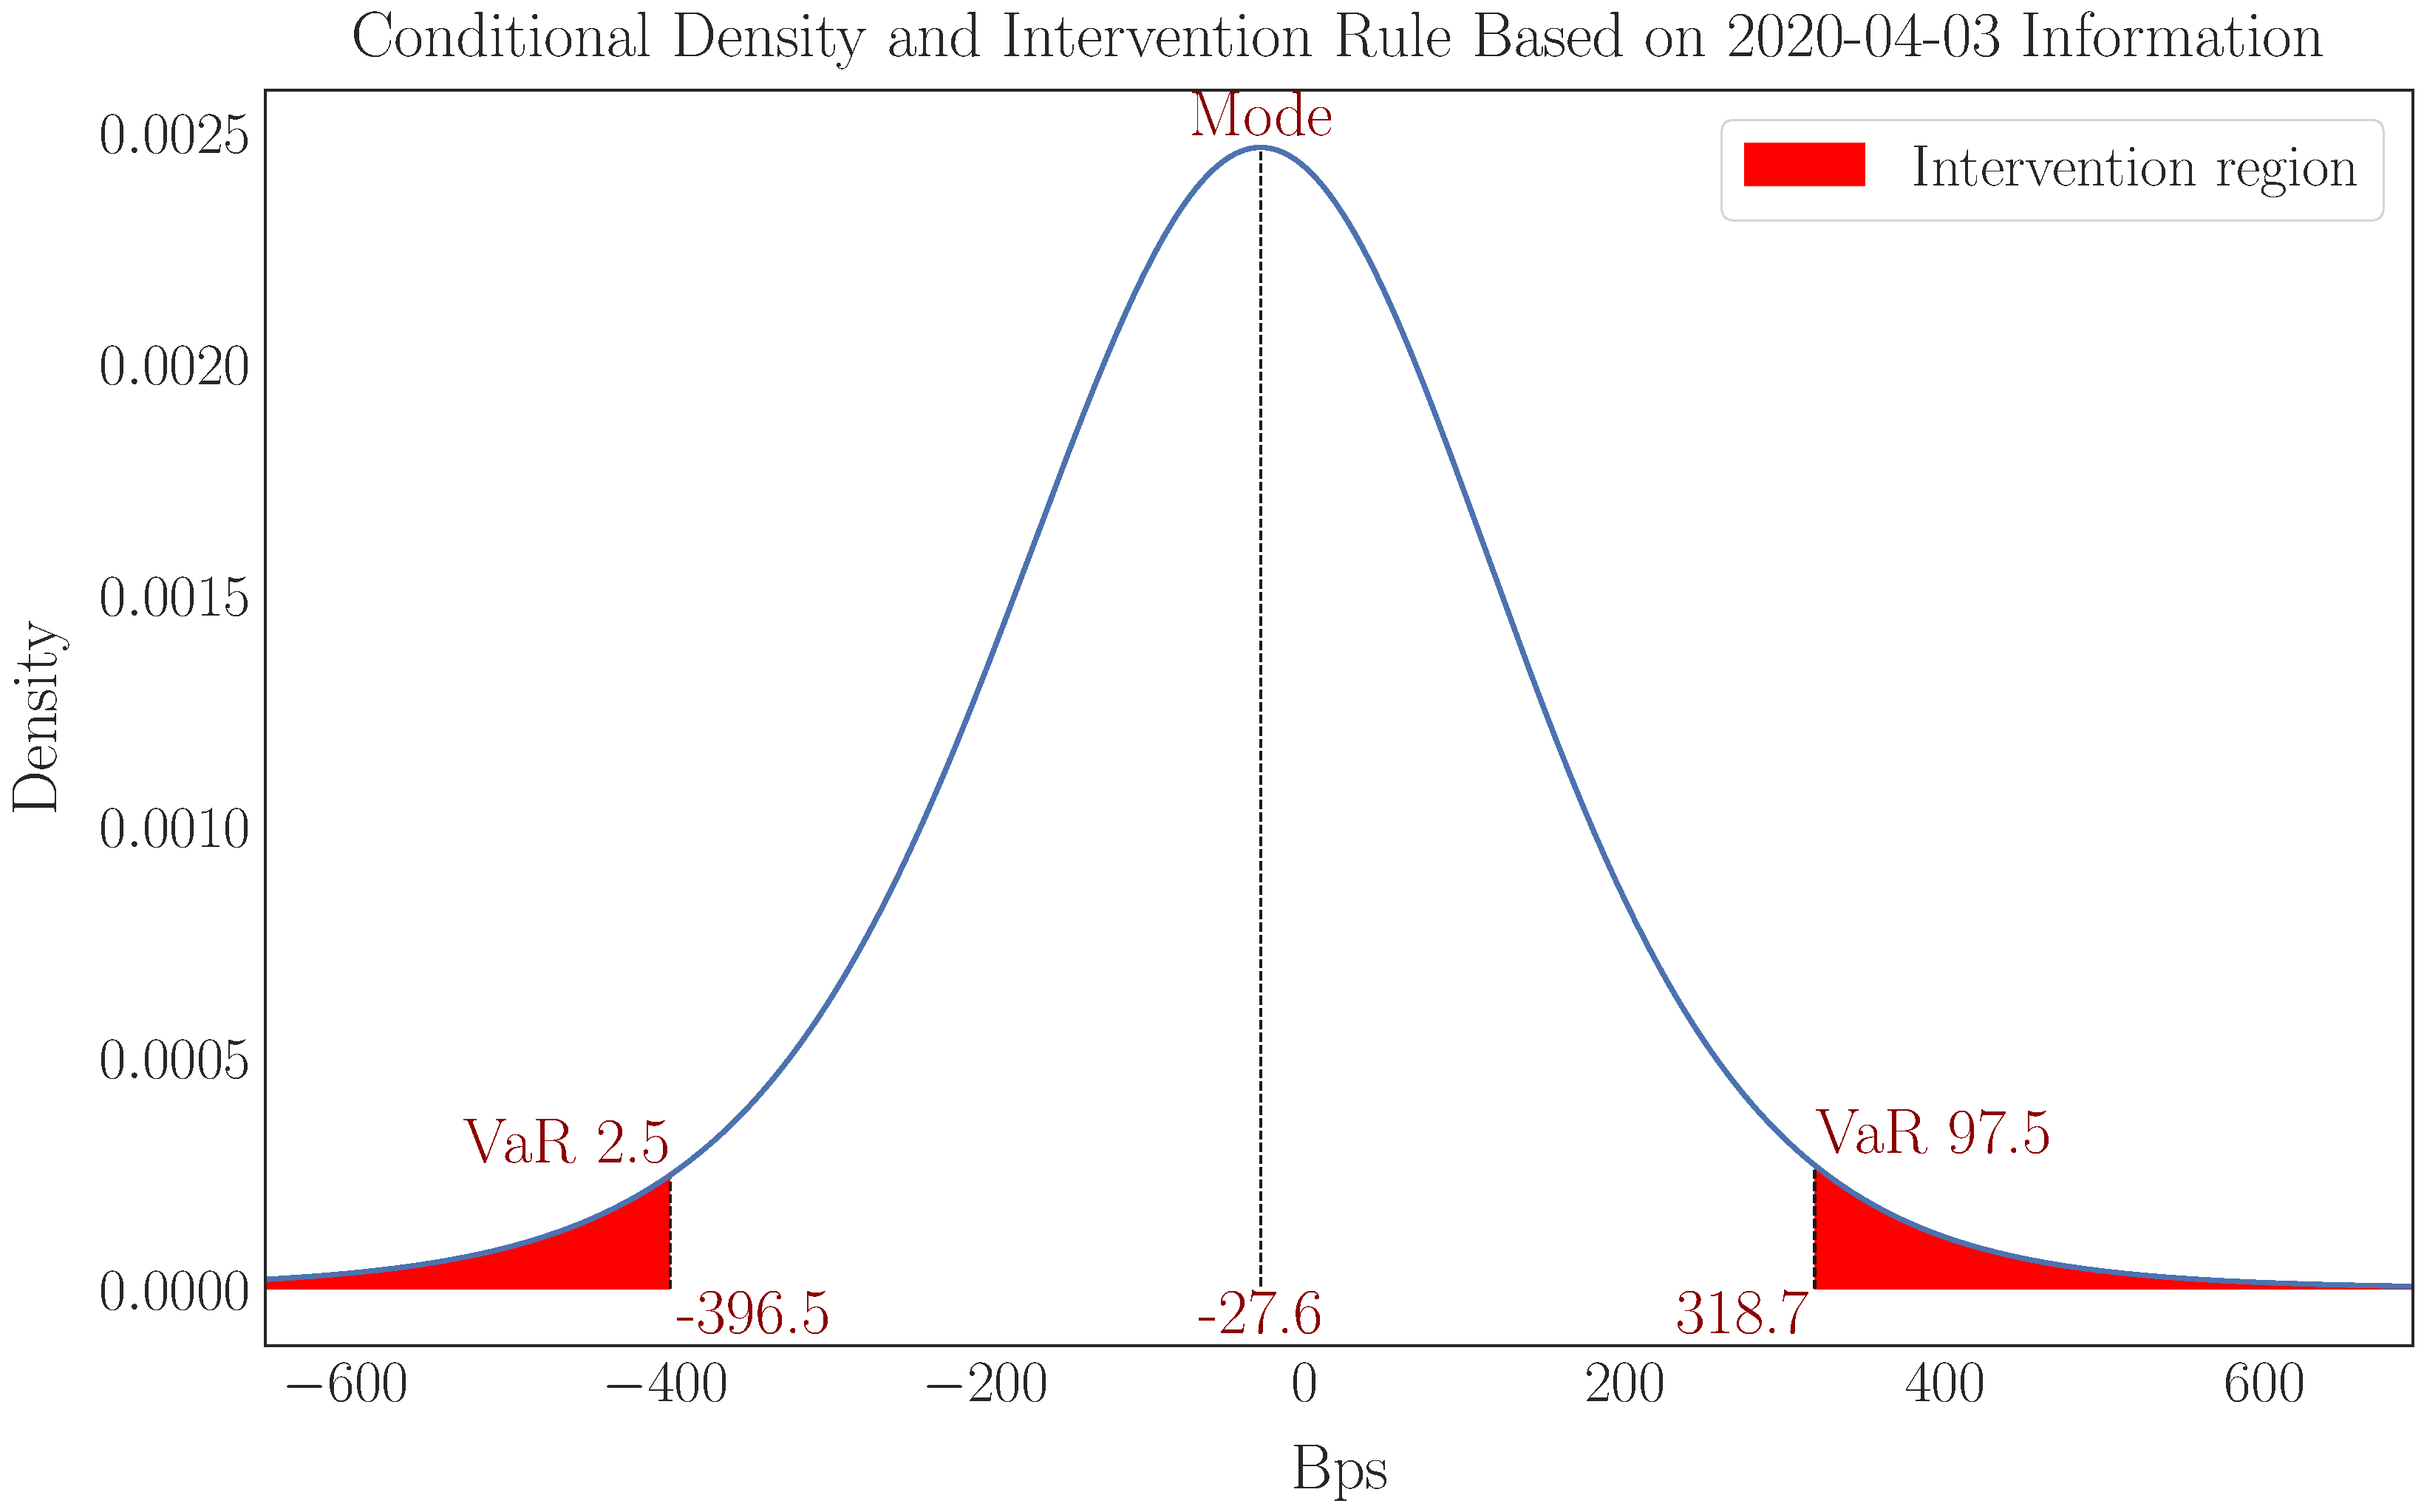
\includegraphics[width=\paperwidth]{img/var_rule.pdf}}
\end{frame}

\begin{frame}
  \frametitle{A Risk-Management Approach to FX Interventions}
  \begin{wideitemize}    
  \item Tail-risks hedge not always available: \textbf{incomplete markets}
    \item \textbf{The central bank is transferring FX risk from the market to
      its balance sheet}. It buys a risky asset (FX) and issues a risk-free asset
      (local currency)    
    \item Provide a \textbf{public good} to address market failure. Leave a
      fix share of risk for the market to hedge 
    \item Risk tolerance should depend on the \textbf{macrofinancial risk} 
    \item The financial stability mandate of the central bank is properly
      formalized and quantified via VaR metric
  \end{wideitemize}  
\end{frame}

\begin{frame}
    \frametitle{Main Features}
  \begin{wideenumerate}
  \item Allows flexible exchange rate to act as a \textbf{shock absorber}:
    more flexibility in crisis time => \textbf{avoid overshooting}
  \item \textbf{No excessive interventions} in crisis time, often ineffective
    and costly (exhaust FX reserves)
  \item No free insurance to the market: avoid \textbf{moral
      hazard}, foster the \textbf{development of hedging market}
  \item Prevent \textbf{market speculation and windfall effects}
  \item Guarantees \textbf{fixed-frequency} interventions: 
    \begin{itemize}
    \item \textbf{Certainty} about interventions: the central bank can intervene with
      \textbf{larger amounts}, more efficient
    \item \textbf{Budget neutrality} with symmetric risk preference
    \end{itemize}
  \item \textbf{Financially optimized}: buy/sell at the best expected price
  \end{wideenumerate}  
\end{frame}


\begin{frame}
  \frametitle{Operational Implementation}
  \begin{wideitemize}
  \item \textbf{Standard data requirements}, easily accessible for a central
    bank, can be customized
  \item Parsimonious GARCH model featuring \textbf{embedded heteroskedasticity},  \textbf{asymmetries}
    (appreciation/depreciation), \textbf{non-linearities} (exponential
    volatility) and parametric \textbf{density forecasting}    
  \item We created a Python package, \textbf{free and open-source}  (available on Github): estimation, forecasting,
    out-of-sample evaluation, optimization, benchmarking, etc. Results are \textbf{fully replicable}
  \item Can be readily used by central banks and deployed during Technical Assistance (TA) missions
  \end{wideitemize}
\end{frame}


\begin{frame}
  \frametitle{Challenges}
  \begin{wideitemize}
      \item Some central banks might be reluctant to use a VaR-rule: \textbf{more
        difficult to communicate} to the public
        \begin{wideitemize}
      \item However, FXI occur on the wholesale FX market, where market
        participants are fully aware of the VaR concept
        \end{wideitemize}        
      \item Some policymakers might \textbf{prefer to keep discretion} over FXI
        \begin{wideitemize}
    \item Trade-off: a transparent rule anchors better market expectations,
      maximize efficiency and strengthen central bank's independence              
        \end{wideitemize}        
  \end{wideitemize}
\end{frame}

\begin{frame}
  \frametitle{The Framework Extends Beyond FXI triggers}    
  \begin{wideenumerate}
    \item Determine FX Intervention triggers
    \item Conduct market monitoring and provide policy guidance
    \item Benchmark FX interventions, including discretionary interventions
    \end{wideenumerate}
    
    \bigskip
    
  \begin{wideitemize}
    \item We present below an application of the toolkit to the Mexican Peso, based on publicly
      available data
    \item More than 4500 daily observations, from 2009 to 2018, with Bank of
      Mexico (public) FX interventions, mostly concentrated in 2009 and 2016
    \end{wideitemize}
    
\end{frame}


%% ---------------------------------------------------------------------------
%% Model
%% ---------------------------------------------------------------------------
\section{Model}

\begin{frame}
  \frametitle{Specification}
\begin{wideitemize}  
\item Non-linear, Exponential GARCH (EGARCH) model 
\item The dependent variable is the FX log-returns, $r_t = \log(\frac{e_t}{e_{t-1}})$, where
$e_t$ is the bilateral market exchange rate against the major currency
(e.g. USD)
\item \textbf{Drift AR-X(1):} $r_{t+1} = \alpha_d +
  \rho r_t + \beta X_{t+1} + \epsilon_{t-1}$\\  
\item \textbf{Exponential volatility:} $\log \sigma_{t+1}^{2} = \omega + \beta
g(r_t)$ where $g(r_t) = \alpha_v r_t + \gamma(|r_t|-\mathbb{E}|r_t|)$

\item \textbf{Error term distribution} $\epsilon_t = \sigma_t \varepsilon_t
  \ , \varepsilon_t \sim \text{TSK}(0, 1,\nu)$\\
  
\item The forecasted conditional probability distribution function is defined as:
      \begin{equation*}
        \hat{f}(r_{t+1} | r_{t}, X_{t+1}) = \text{TSK}(\hat{r}_{t+1},
        \hat{\sigma}_{t+1}^{2}, \hat{\nu})
      \end{equation*}      
\end{wideitemize}
\end{frame}

% Estimation
\begin{frame}{Estimation}
\begin{wideitemize}
\item The GARCH estimation is standard and done with maximimum likelihood
 \item Selection of parameters is done via AIC/BIC criteria.    
  \item Our Python package allows to flexibly select:
    \begin{itemize}
    \item The set of exogeneous regressors
    \item The number of lags
    \item The volatility specification (exponential, RiskMetric, standard GARCH,
      etc.)
    \item The distribution family of the error-terms (Gaussian,
    Student, Tskew, Generalized Gaussian, etc.)  
  \end{itemize}
\item More complex models (e.g. copulas, non-parametric kernels, etc.) can be
  used within the same VaR framework. However, more difficult to understand
  and to implement
\end{wideitemize}
\end{frame}

\begin{frame}{Exogeneous Regressors}
  \begin{wideenumerate}
  \item \textbf{FX microstructure}: FX bid-ask spread (averaged over the day)
  \item \textbf{CIP}: daily interest rate differential with the US Libor 
  \item \textbf{Hedging costs}: one-month forward exchange rate
  \item \textbf{Past policy interventions}: lagged amount of central bank FX intervention 
  \item \textbf{Global risk sentiment}: The VIX, implied volatility on the S\&P 500 
  \item \textbf{Global FX factor}: The EURUSD exchange rate
  \end{wideenumerate}
 
\end{frame}


\begin{frame}{Regression Table}
\setlength\tabcolsep{2pt}  % default value: 6pt
\tiny  %%  command to change the font size
\begin{tabular}{llllll}
\toprule
{} & Microstructure &       CIP & Dollar move & Risk Appetite &  Baseline \\
\midrule
Intercept                       &          -2.34 &     -2.29 &       -1.74 &         -2.55 &     -1.63 \\
Lag FX log returns              &       -0.07*** &  -0.08*** &    -0.08*** &      -0.08*** &  -0.08*** \\
Bid ask abs                     &           5.67 &     24.45 &      -33.58 &         -2.68 &      3.22 \\
Min max abs                     &          35.62 &     34.68 &       33.32 &        34.45* &      26.2 \\
Forward points first difference &       23.29*** &  17.79*** &    26.33*** &      19.82*** &  19.44*** \\
Interbank rate vs Libor         &                &  33.61*** &    39.43*** &      34.75*** &  33.86*** \\
EURUSD log returns              &                &           &    -0.14*** &      -0.17*** &  -0.16*** \\
VIX first diff                  &                &           &             &      15.67*** &  15.37*** \\
FX intervention dummy lag       &                &           &             &               &      2.23 \\
Oil prices log returns          &                &           &             &               &  -0.02*** \\
Omega                           &        0.13*** &   0.13*** &     0.12*** &       0.11*** &   0.12*** \\
Alpha                           &        0.17*** &   0.17*** &     0.16*** &       0.16*** &   0.15*** \\
Gamma                           &        0.07*** &   0.06*** &     0.06*** &       0.05*** &   0.05*** \\
Beta                            &        0.98*** &   0.99*** &     0.99*** &       0.99*** &   0.99*** \\
Nu                              &        8.33*** &   8.67*** &     8.92*** &       8.71*** &   8.54*** \\
Lambda                          &          0.08* &      0.07 &       0.09* &         0.07* &   0.08*** \\
R2                              &          5.8 \% &     6.7 \% &      10.4 \% &        27.3 \% &    27.6 \% \\
R2 adjusted                     &          5.8 \% &     6.6 \% &      10.3 \% &        27.2 \% &    27.5 \% \\
Number of observations          &           5986 &      5986 &        5682 &          5682 &      5680 \\
Significance *10\%, **5\%, ***1\%  &                &           &             &               &           \\
\bottomrule
\end{tabular}

\normalsize
\end{frame}

\begin{frame}{Formalization of the Intervention Rule}
  \begin{wideitemize}
    \item Consider the estimated conditional distribution of the exchange rate log
      returns $r_t$ defined as
      \begin{equation*}
      \mathbb{P}[r_t \leq x] = \int_{-\infty}^{x}\hat{f}(r_t | r_{t-1}, X_t)
      dr_t        
      \end{equation*}
    \item The Conditional Value-at-Risk at threshold $\tau$ is simply defined as
      the conditional $\tau$-quantile
      \begin{equation*}
      Q(r_t, \tau) \equiv  \mathbb{P}[r_t
      \leq Q(r_t, \tau)] = \tau, \ \text{for} \ \tau \in (0,1)
      \end{equation*}        
    \item The FXI intervention rule is a simple boolean rule, based on two
      risk-thresholds ($\underline{\tau}, \overline{\tau}$), for depreciation
      and appreciation, potentially risk-symmetric ($\overline{\tau} = 1 - \underline{\tau}$)
      \begin{equation*}
\mathbbm{1} \left[ \{r_t \leq \ Q(r_t, \underline{\tau})\} \cup \{r_t > \
  Q(r_t, \overline{\tau})\} \right]
      \end{equation*}                
  \end{wideitemize}
  
\end{frame}

\begin{frame}
\frametitle{Dynamics of the Mexican Peso against USD}
    \makebox[\linewidth]{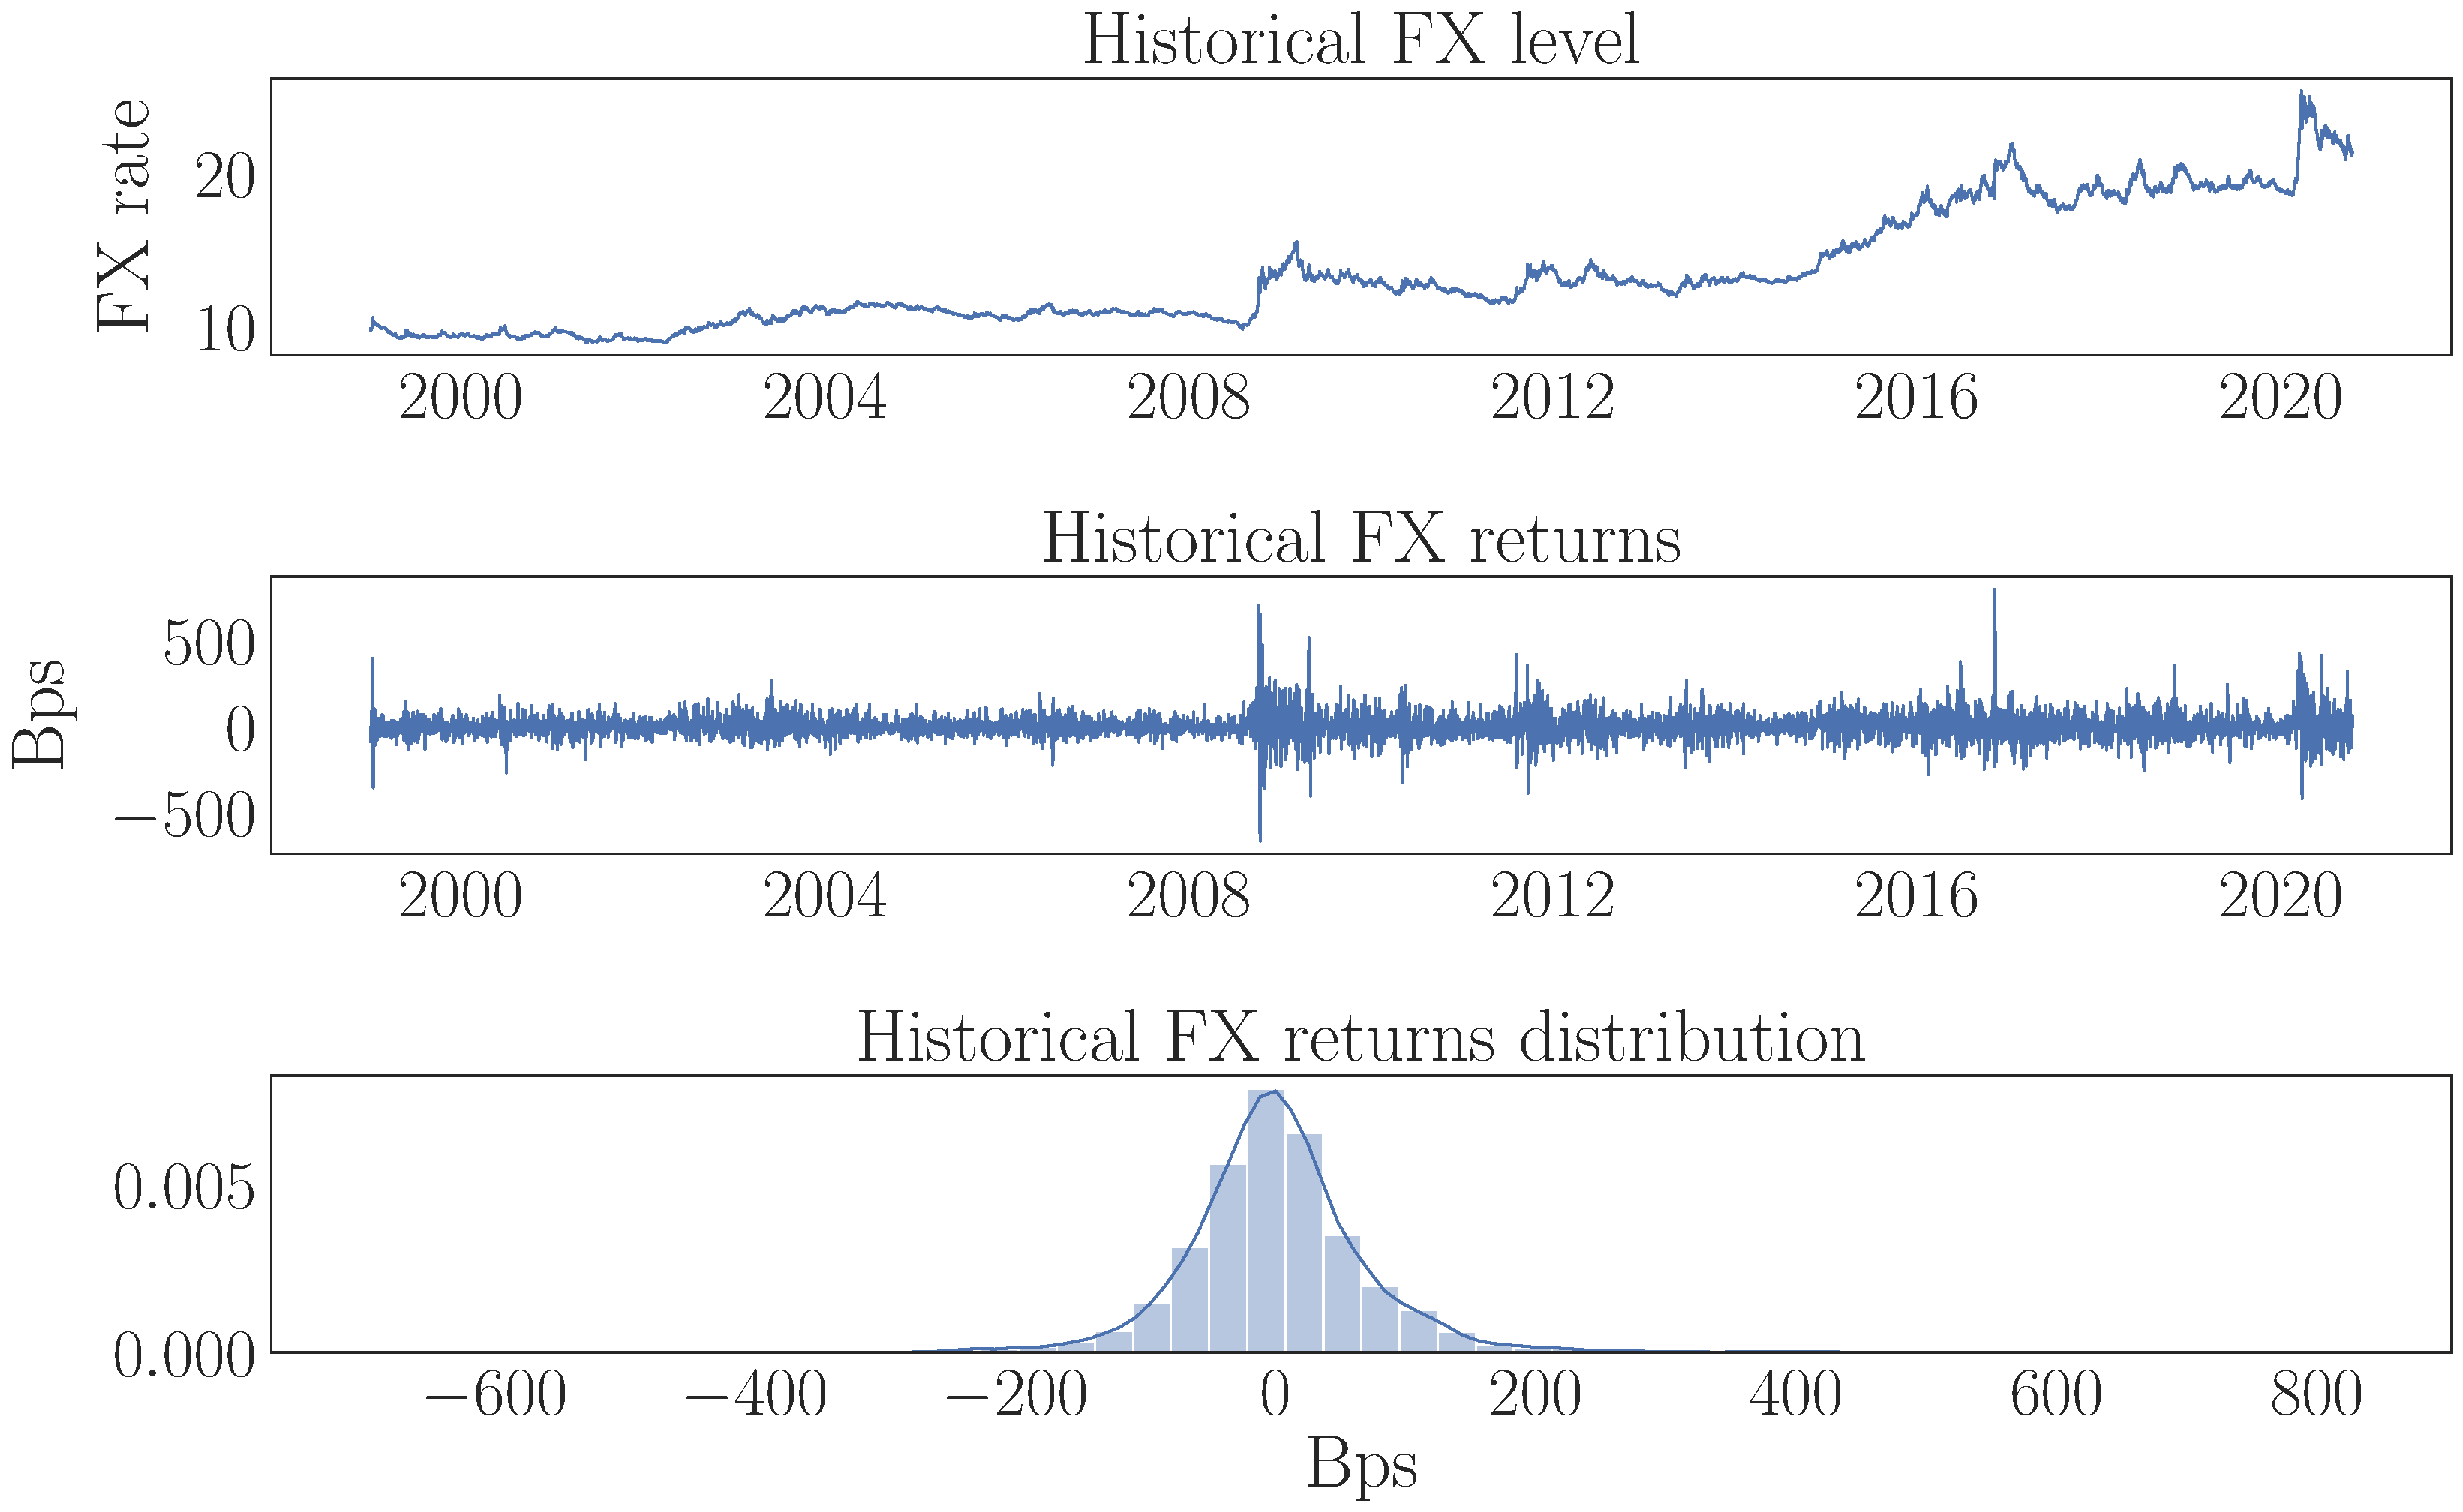
\includegraphics[width=\paperwidth]{img/descriptive_plot.pdf}}
\end{frame}

\begin{frame}
\frametitle{Conditional In-Sample Volatility of the Mexican Peso}
    \makebox[\linewidth]{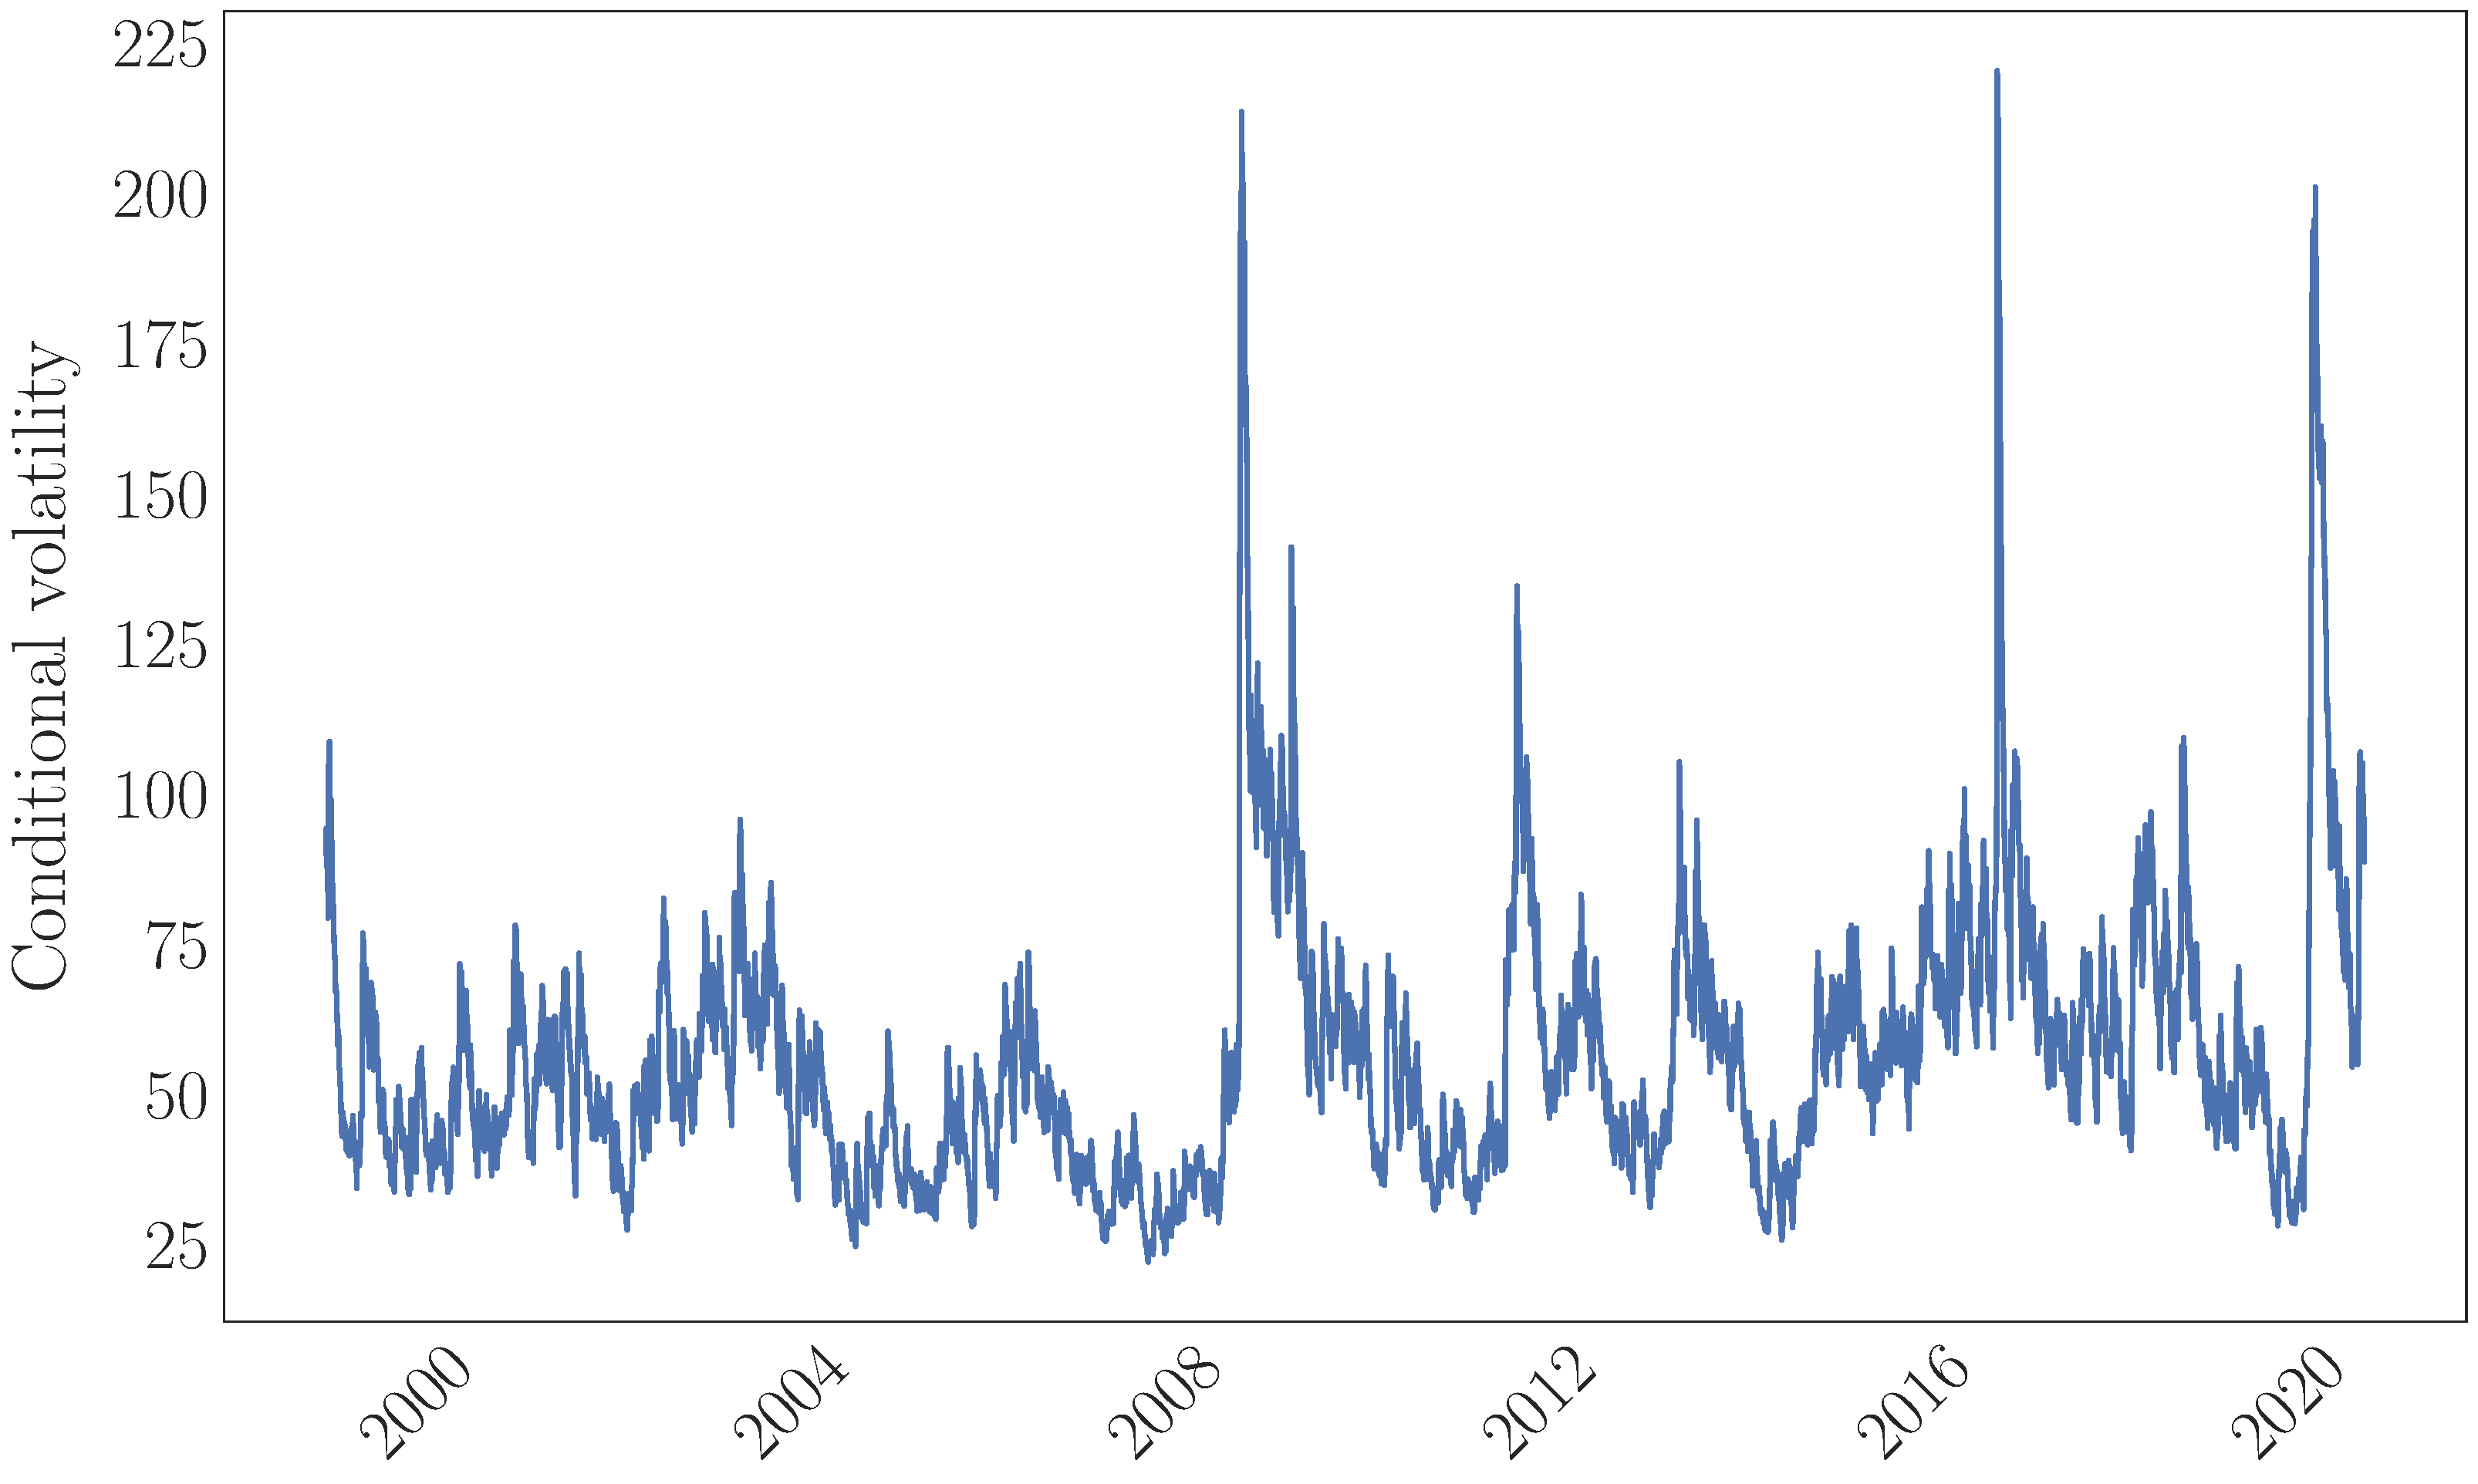
\includegraphics[width=\paperwidth]{img/conditional_vol_plot.pdf}}
\end{frame}

%% ---------------------------------------------------------------------------
%% Forecasting
%% ---------------------------------------------------------------------------
\section{Forecasting}

\begin{frame}
  \frametitle{Forecasting}

  \begin{wideitemize}
      \item Real-time forecasting based on market conditions
    \item Estimate the GARCH and derive the forecasted drift and volatility
    \item Infer the \textbf{full-fledged conditional distribution} of FX log returns for any point
      in time
    \item Optimize the choice of the mean (drift) and density models, specifically:
      \begin{itemize}
      \item The model on the mean/drift
      \item The model for the conditional variance
      \item The distribution of the perturbations, that determines the whole distribution      
      \end{itemize}
  \end{wideitemize}  
\end{frame}



\begin{frame}
\makebox[\linewidth]{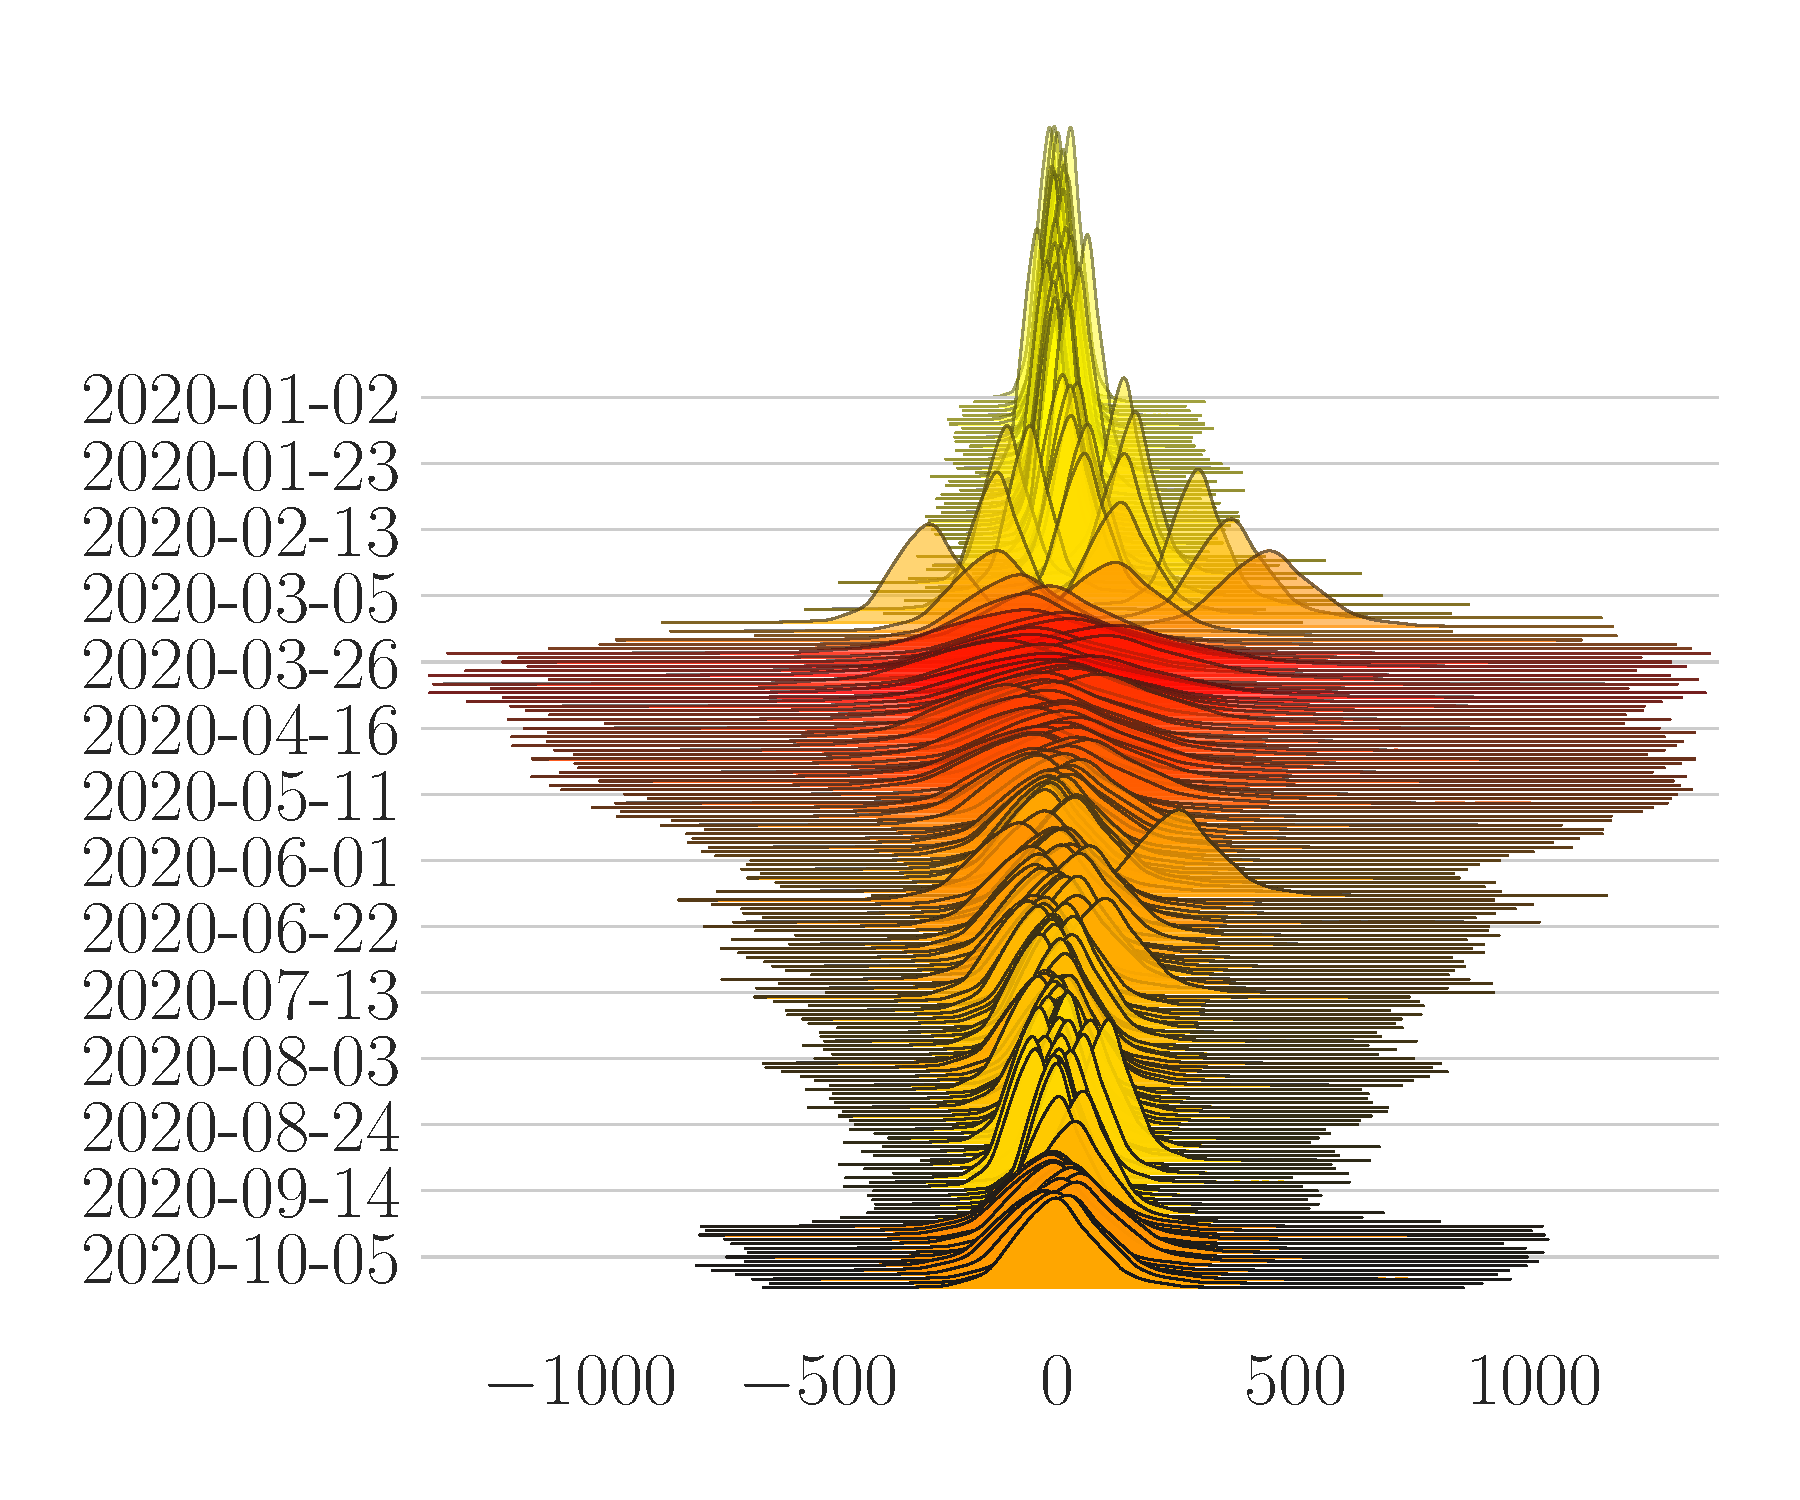
\includegraphics[width=\paperwidth, height=\paperheight]{img/joyplot.pdf}}
\end{frame}

\begin{frame}
 \frametitle{Fan Chart}
\makebox[\linewidth]{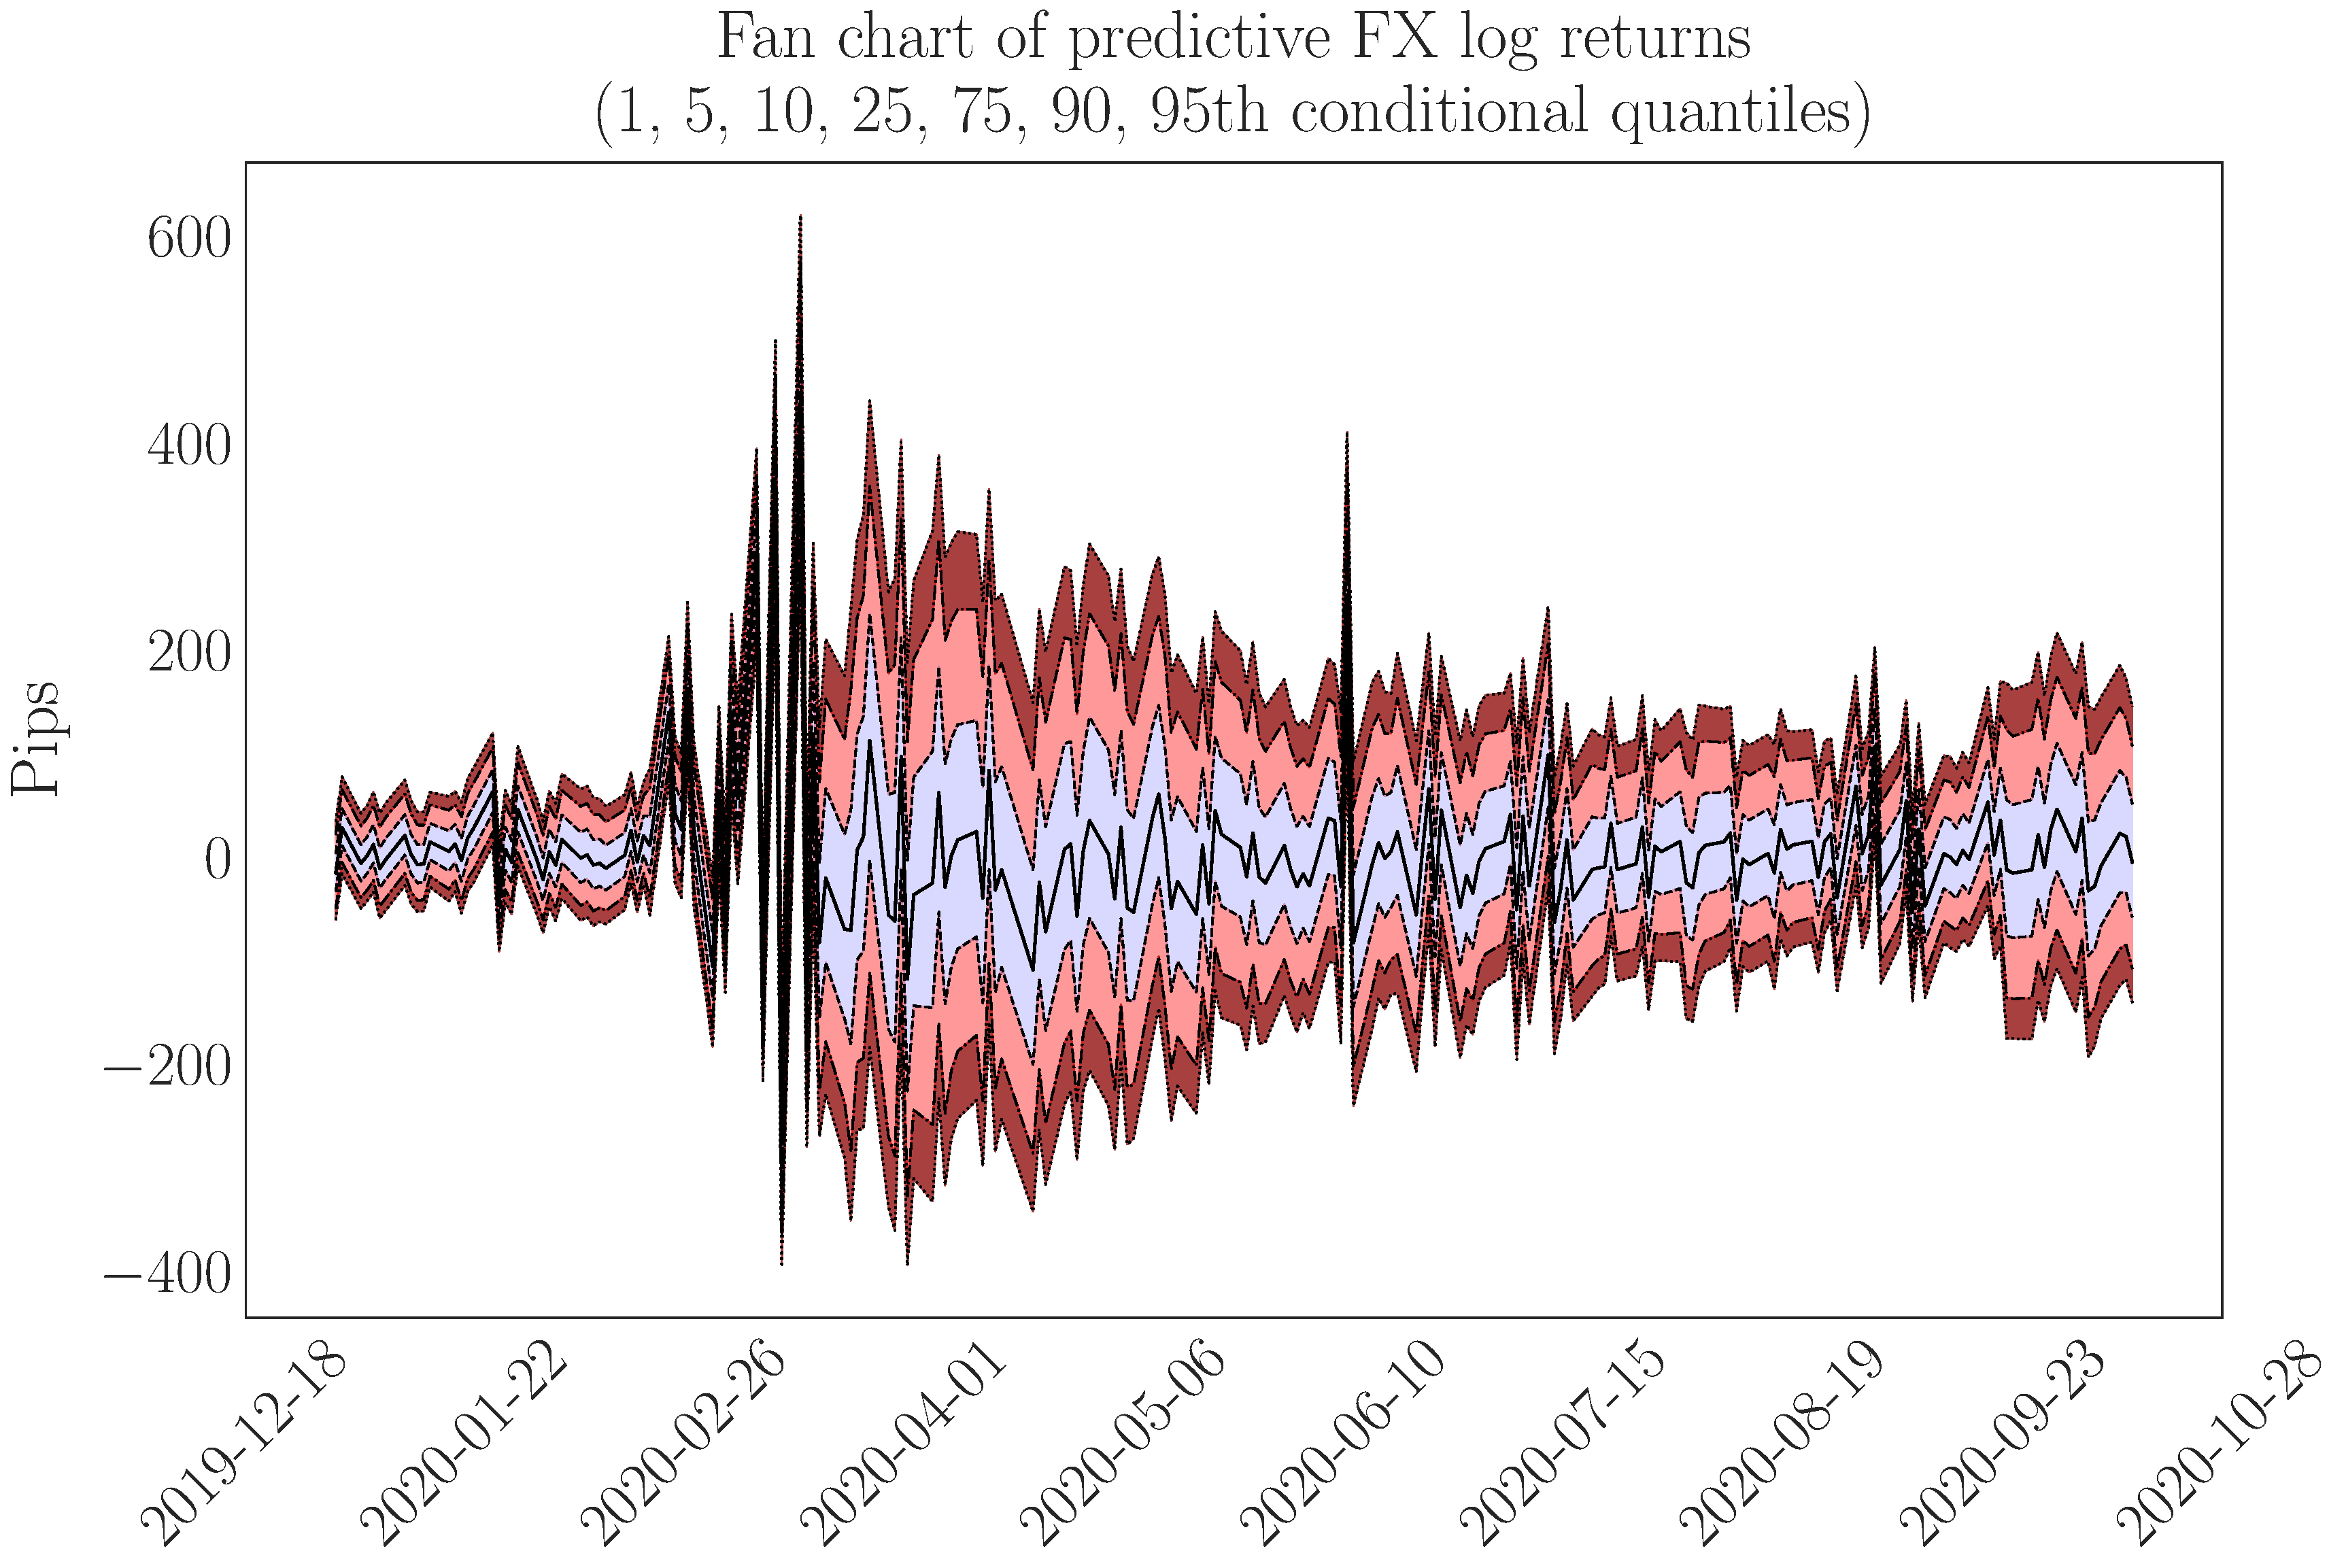
\includegraphics[width=0.95\paperwidth]{img/fanchart.pdf}}
\end{frame}

\begin{frame}
  \frametitle{VaR FXI Rule}
    \makebox[\linewidth]{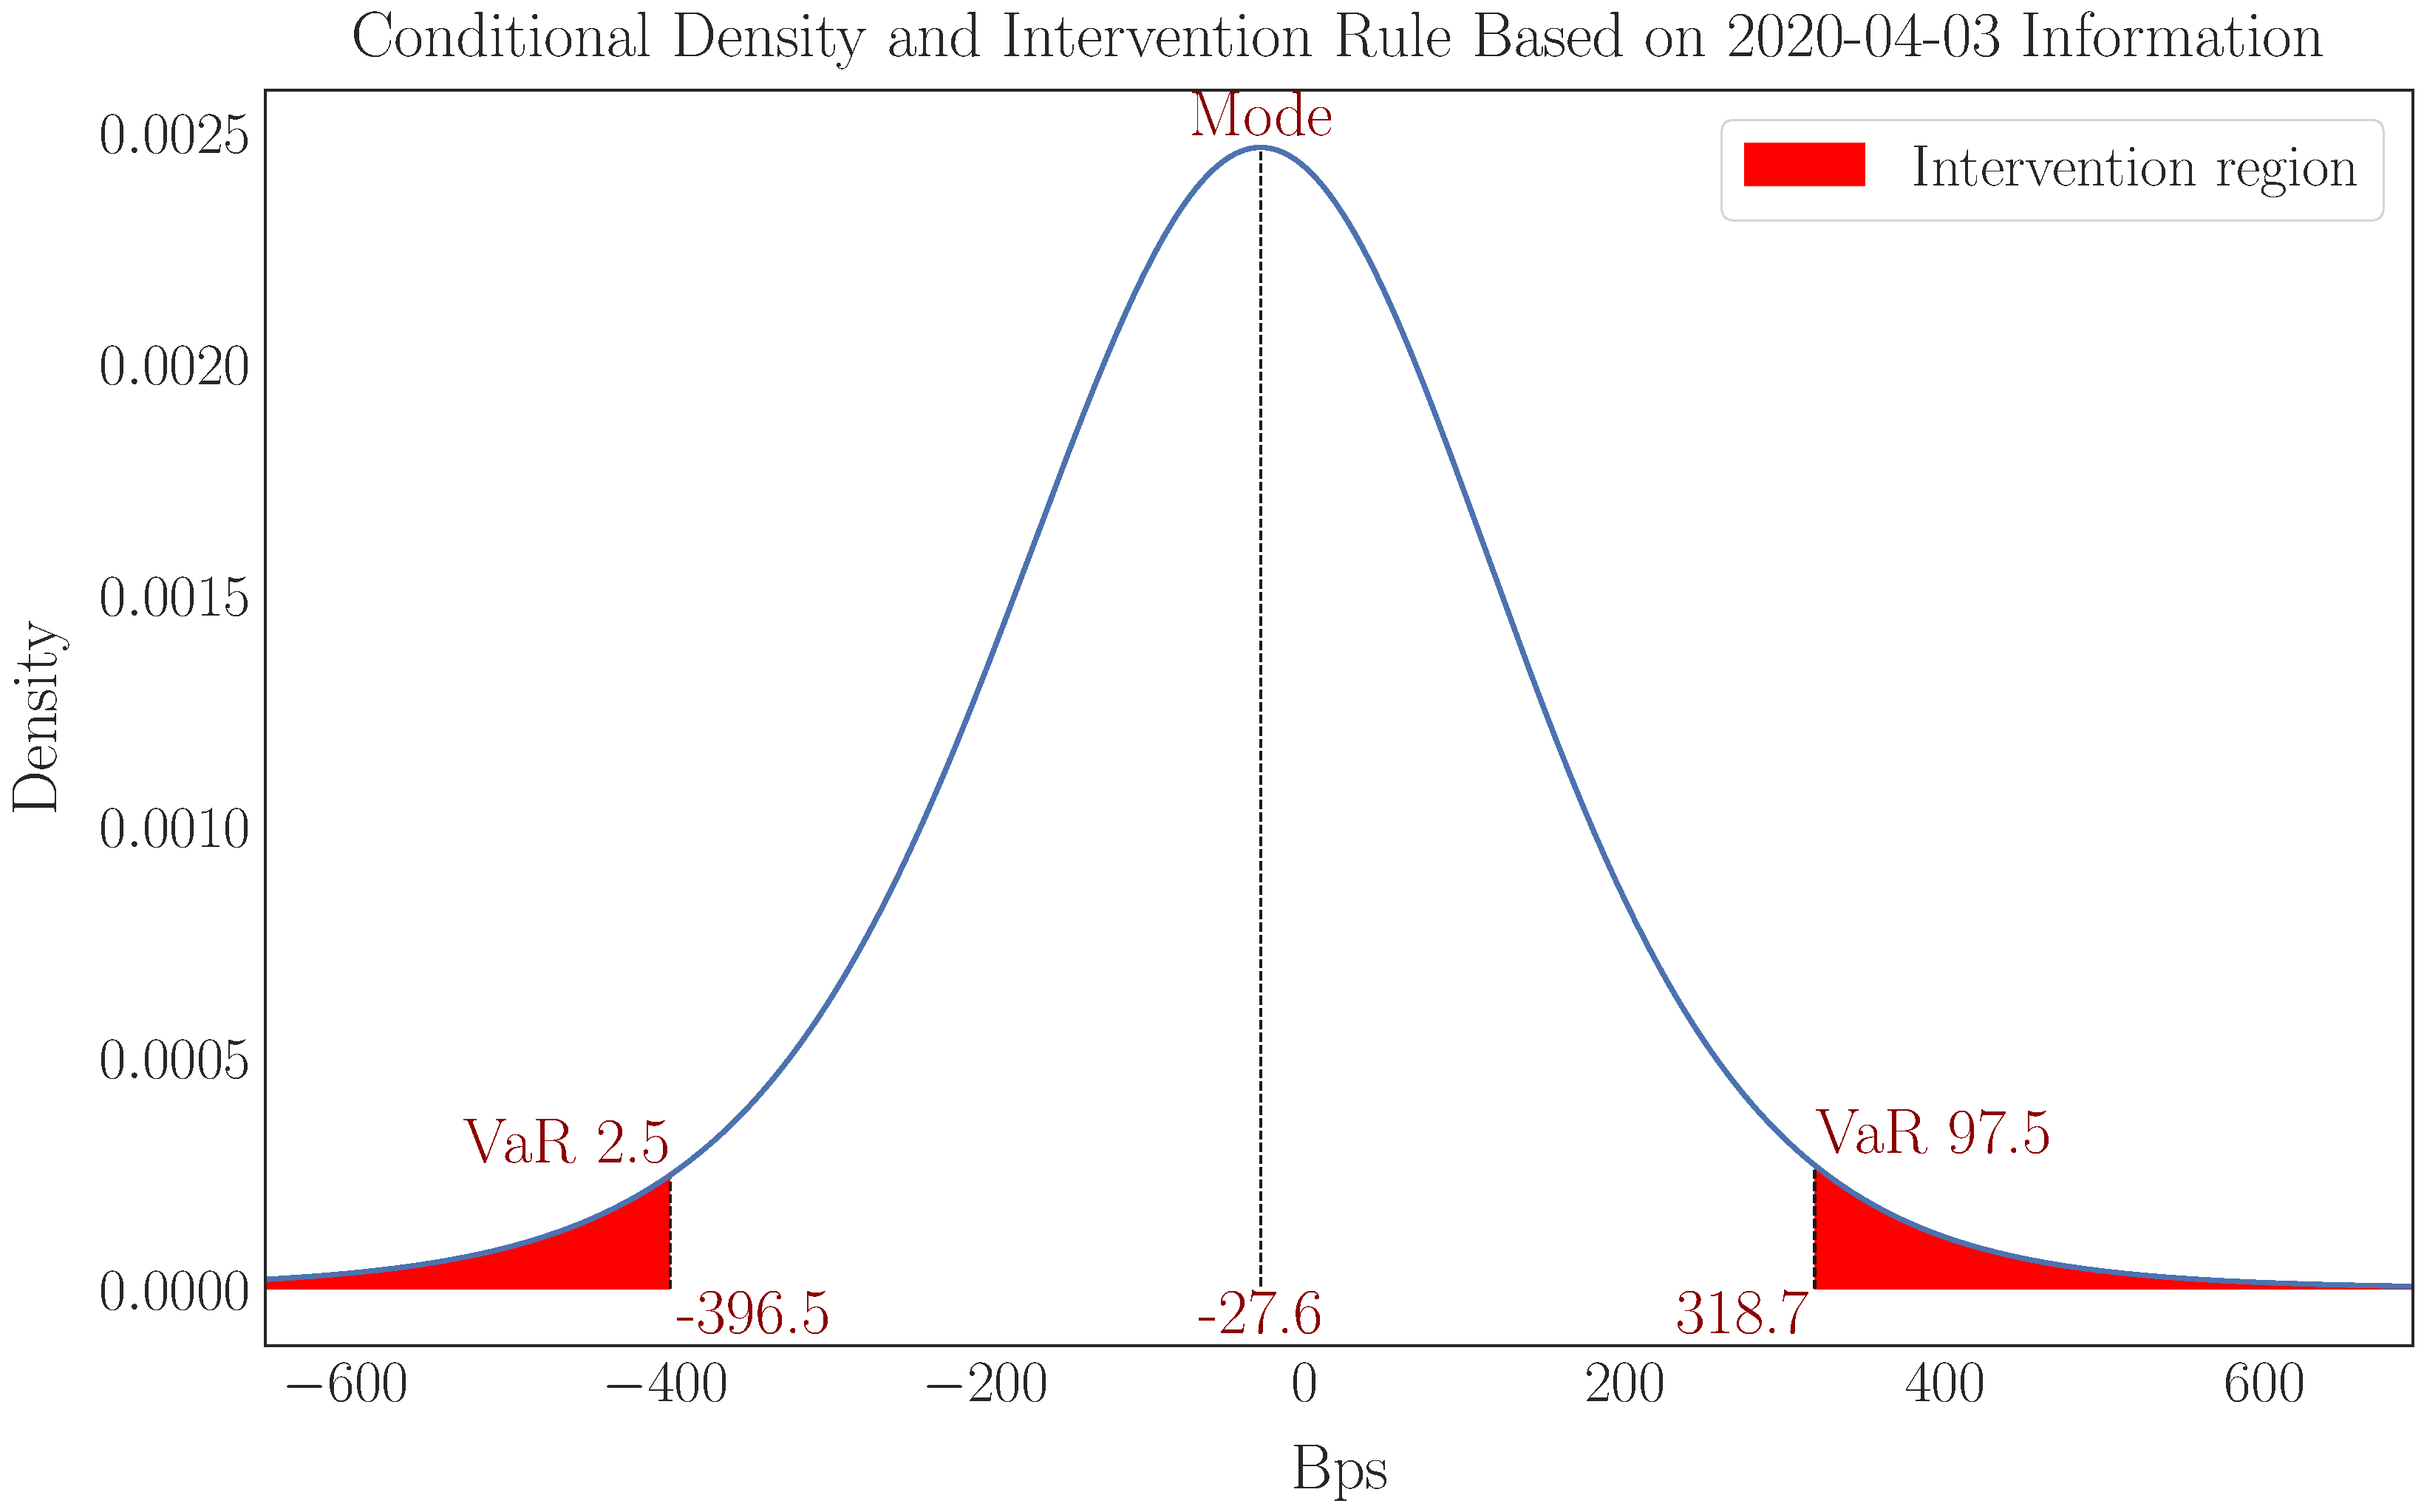
\includegraphics[width=\paperwidth]{img/var_rule.pdf}}
\end{frame}

\begin{frame}
  \frametitle{Conditional Cumulative Distribution Function}
    \makebox[\linewidth]{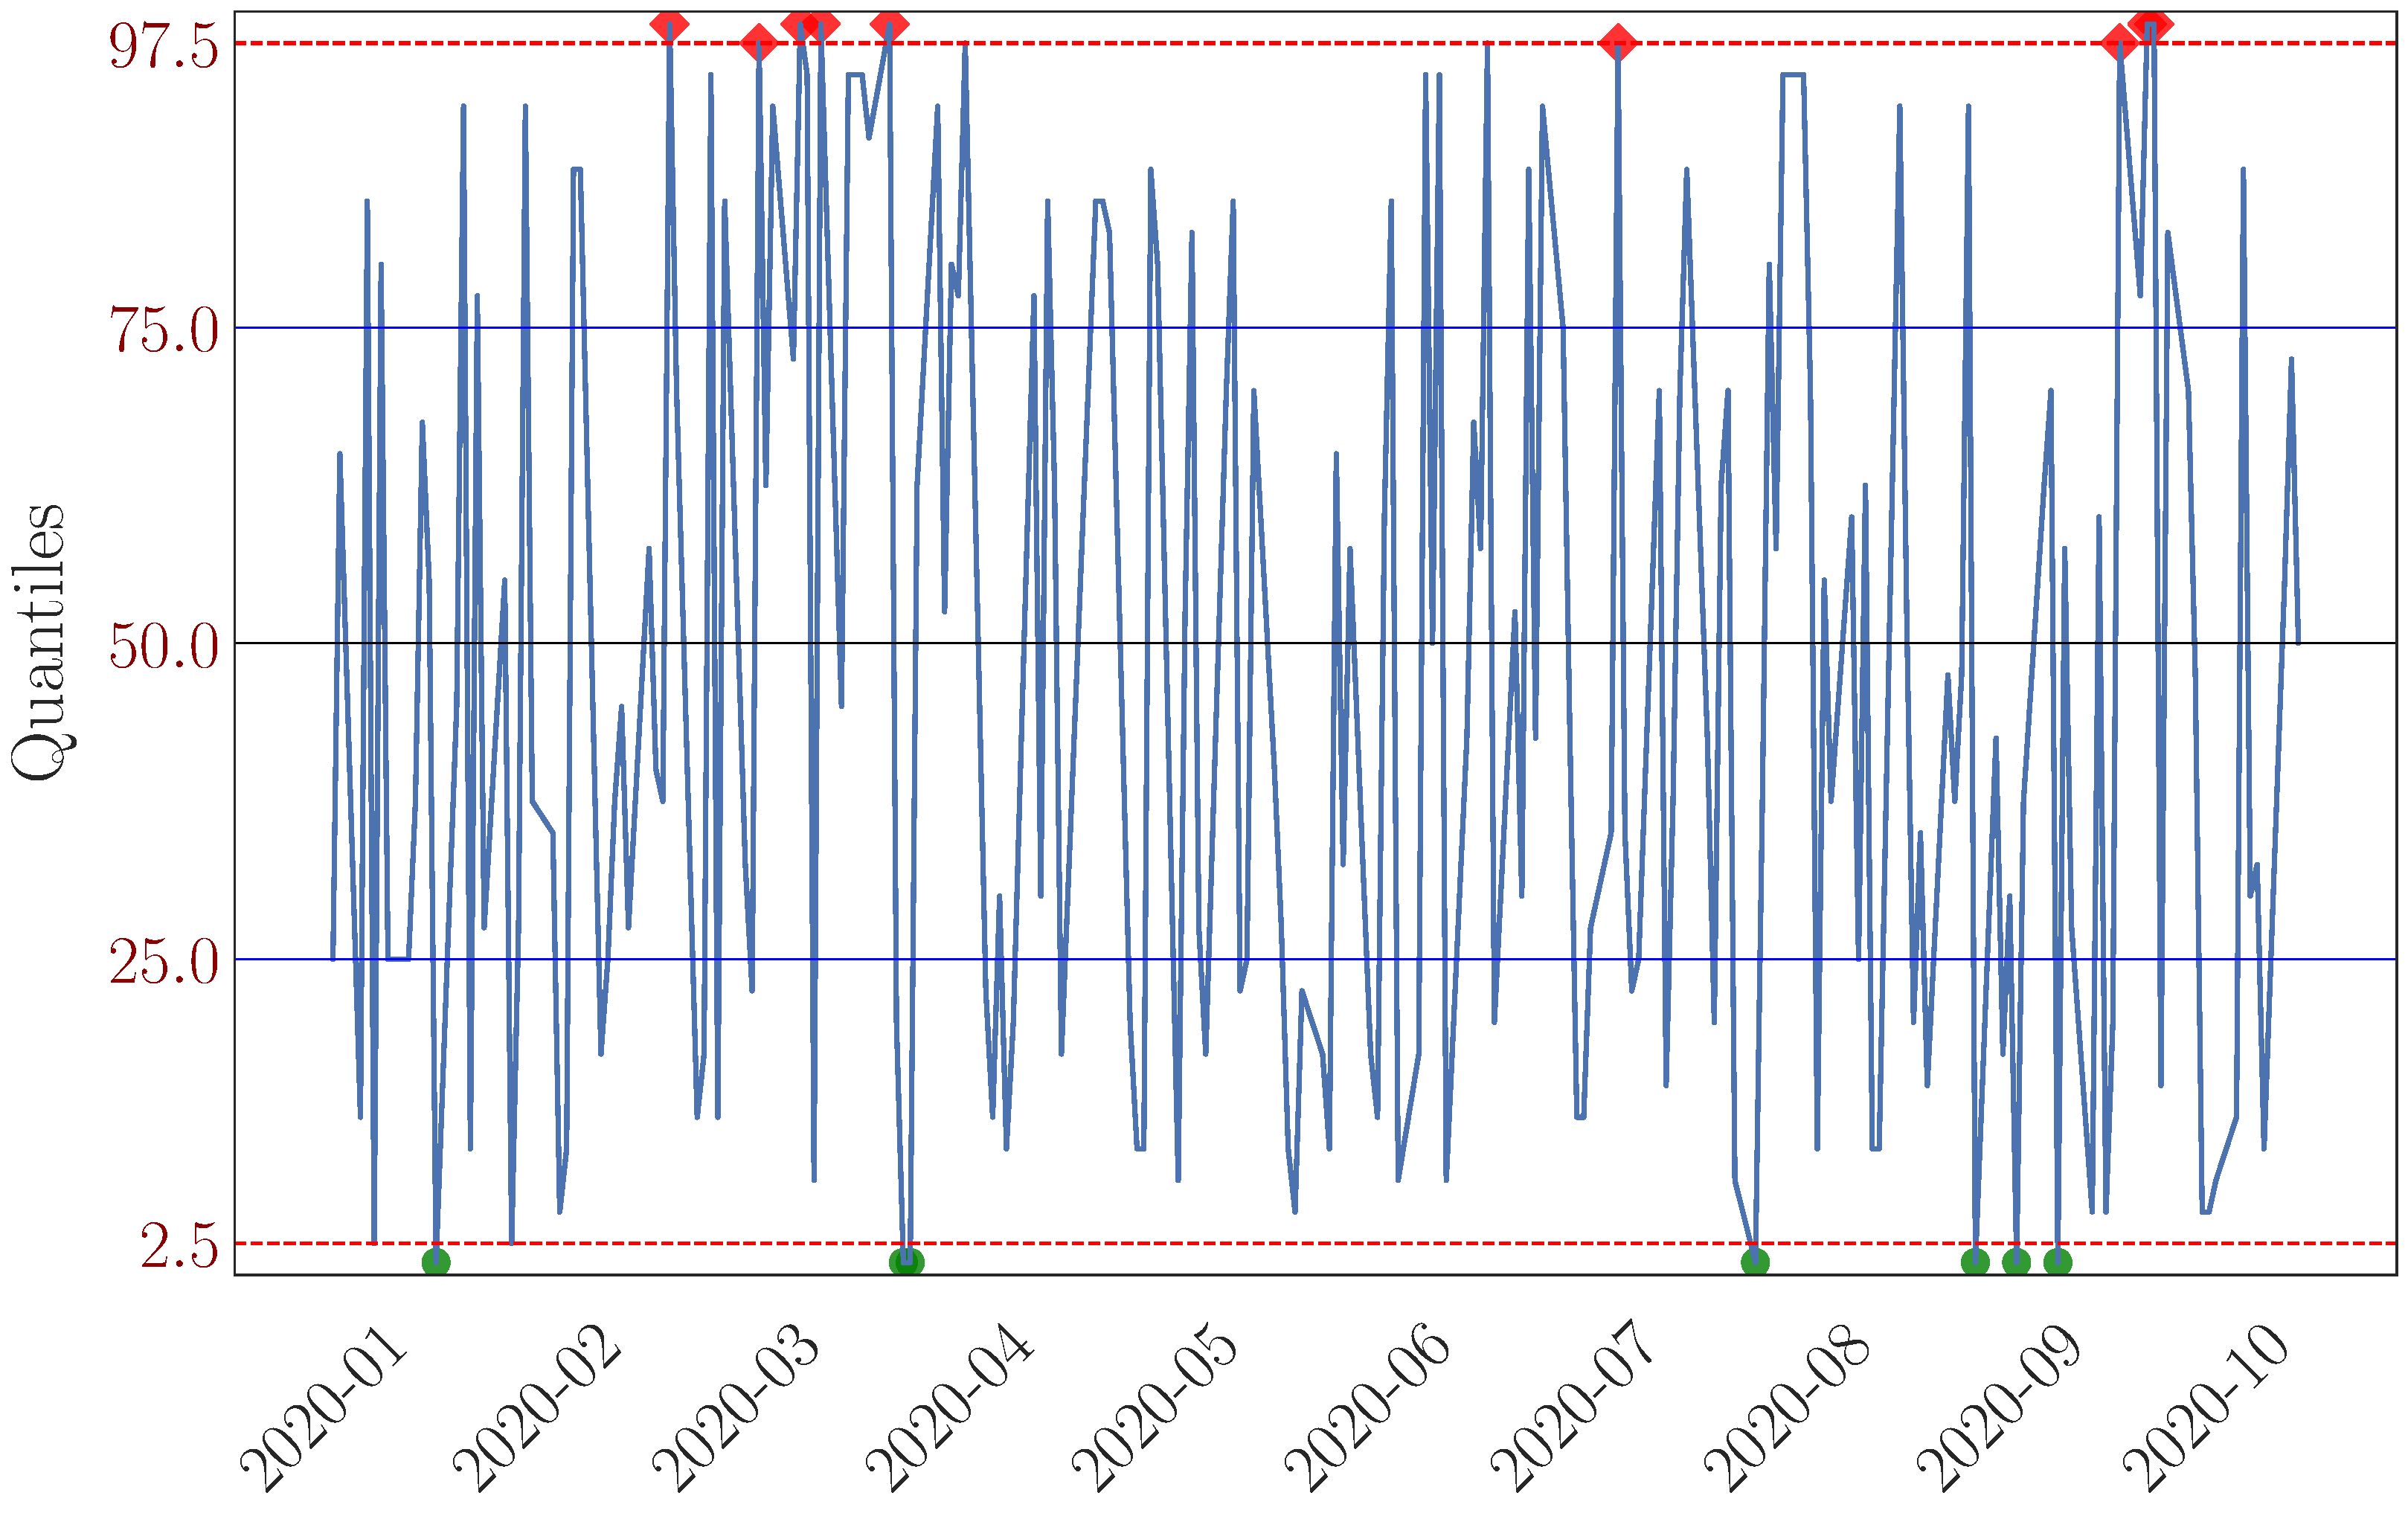
\includegraphics[width=\paperwidth]{img/conditional_cdf.pdf}}
\end{frame}

\begin{frame}
  \frametitle{Conditional Exceedance}
    \makebox[\linewidth]{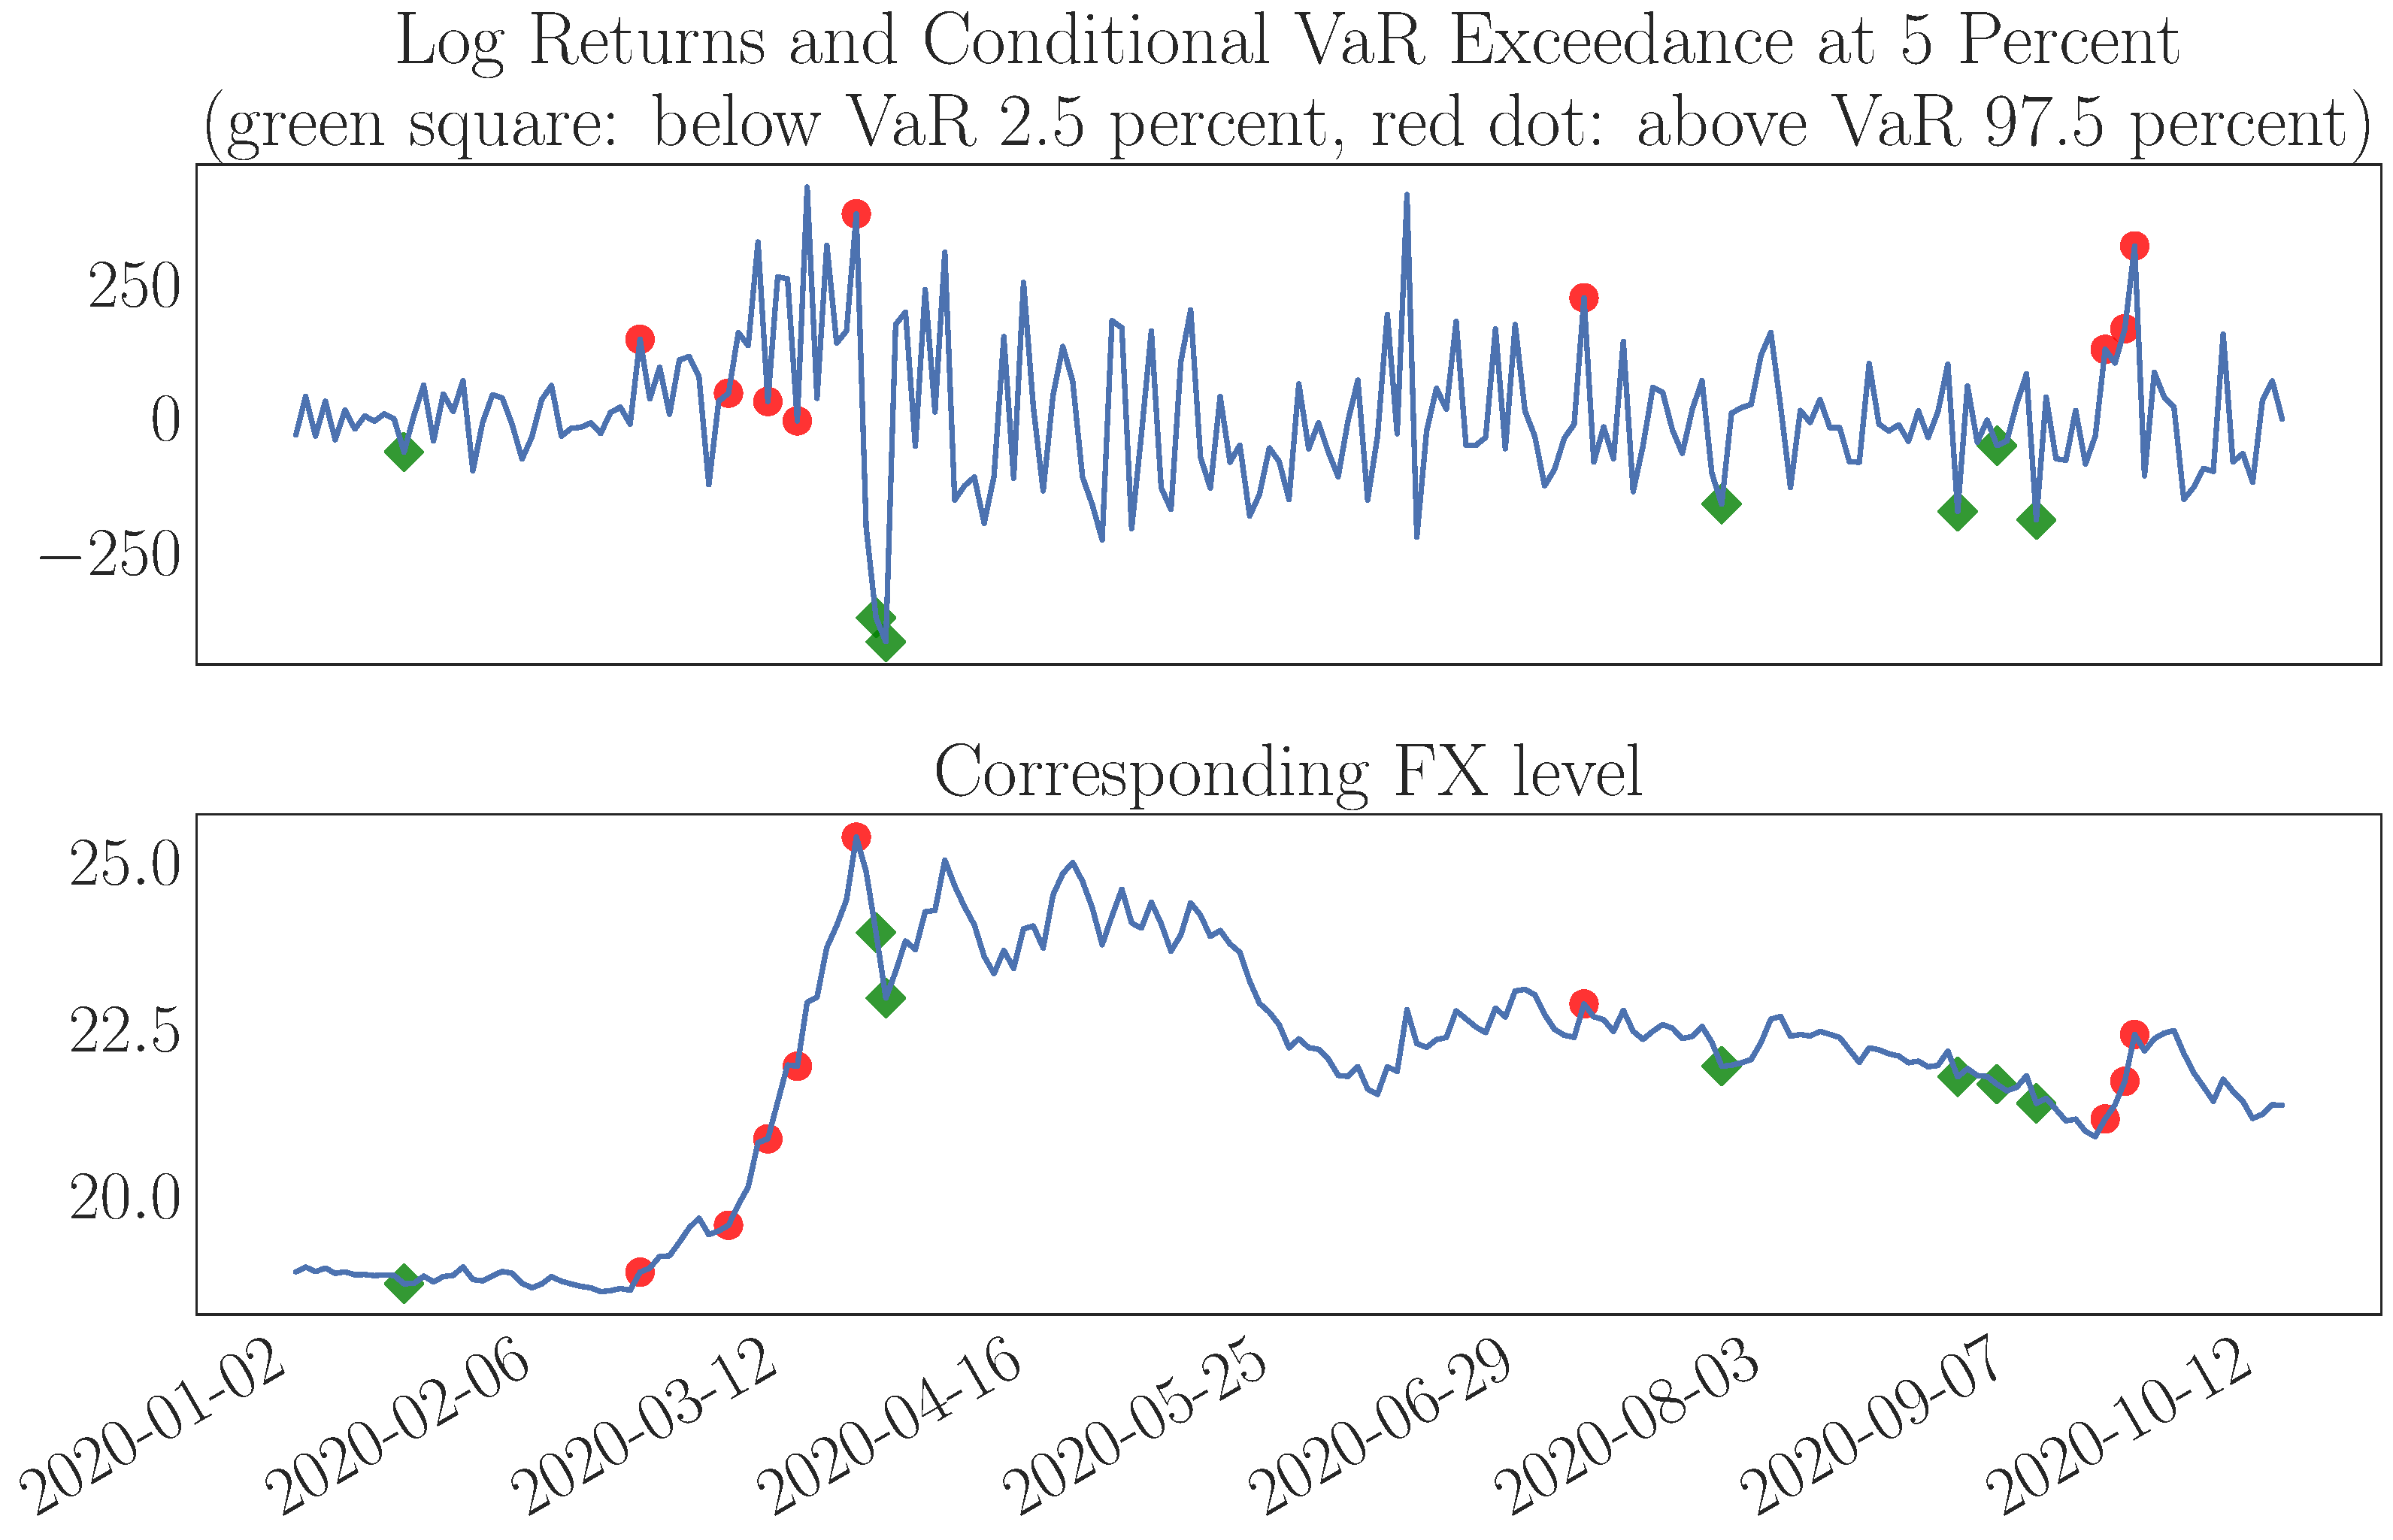
\includegraphics[width=\paperwidth]{img/conditional_exceedance.pdf}}
\end{frame}


\begin{frame}
  \frametitle{Optimization via Cross-Validation using the Zig-Zag Algorithm}
  \begin{wideitemize}
    \item There are many possible choices for the models on the mean/drift, the conditional variance or the distribution of the perturbations
    \item We would like to choose the most appropriate ones, using performance metrics
    \item Problem: the GARCH estimates separately the drift and the volatility (where it imposes assumptions on the distribution)
    \item Idea: use the zig-zag algorithm to optimize the entire model
      \begin{enumerate}
      \item Optimize the choice of the drift model with RMSE out-of-sample validation 
      \item Optimize the choice of the distribution
      \item Estimate the parameters based on the optimal functional forms of the models (the hyperparameters) via a recursive approach
      \end{enumerate}      
  \end{wideitemize}  
\end{frame}

     
\begin{frame}
  \frametitle{Density Evaluation}
    \makebox[\linewidth]{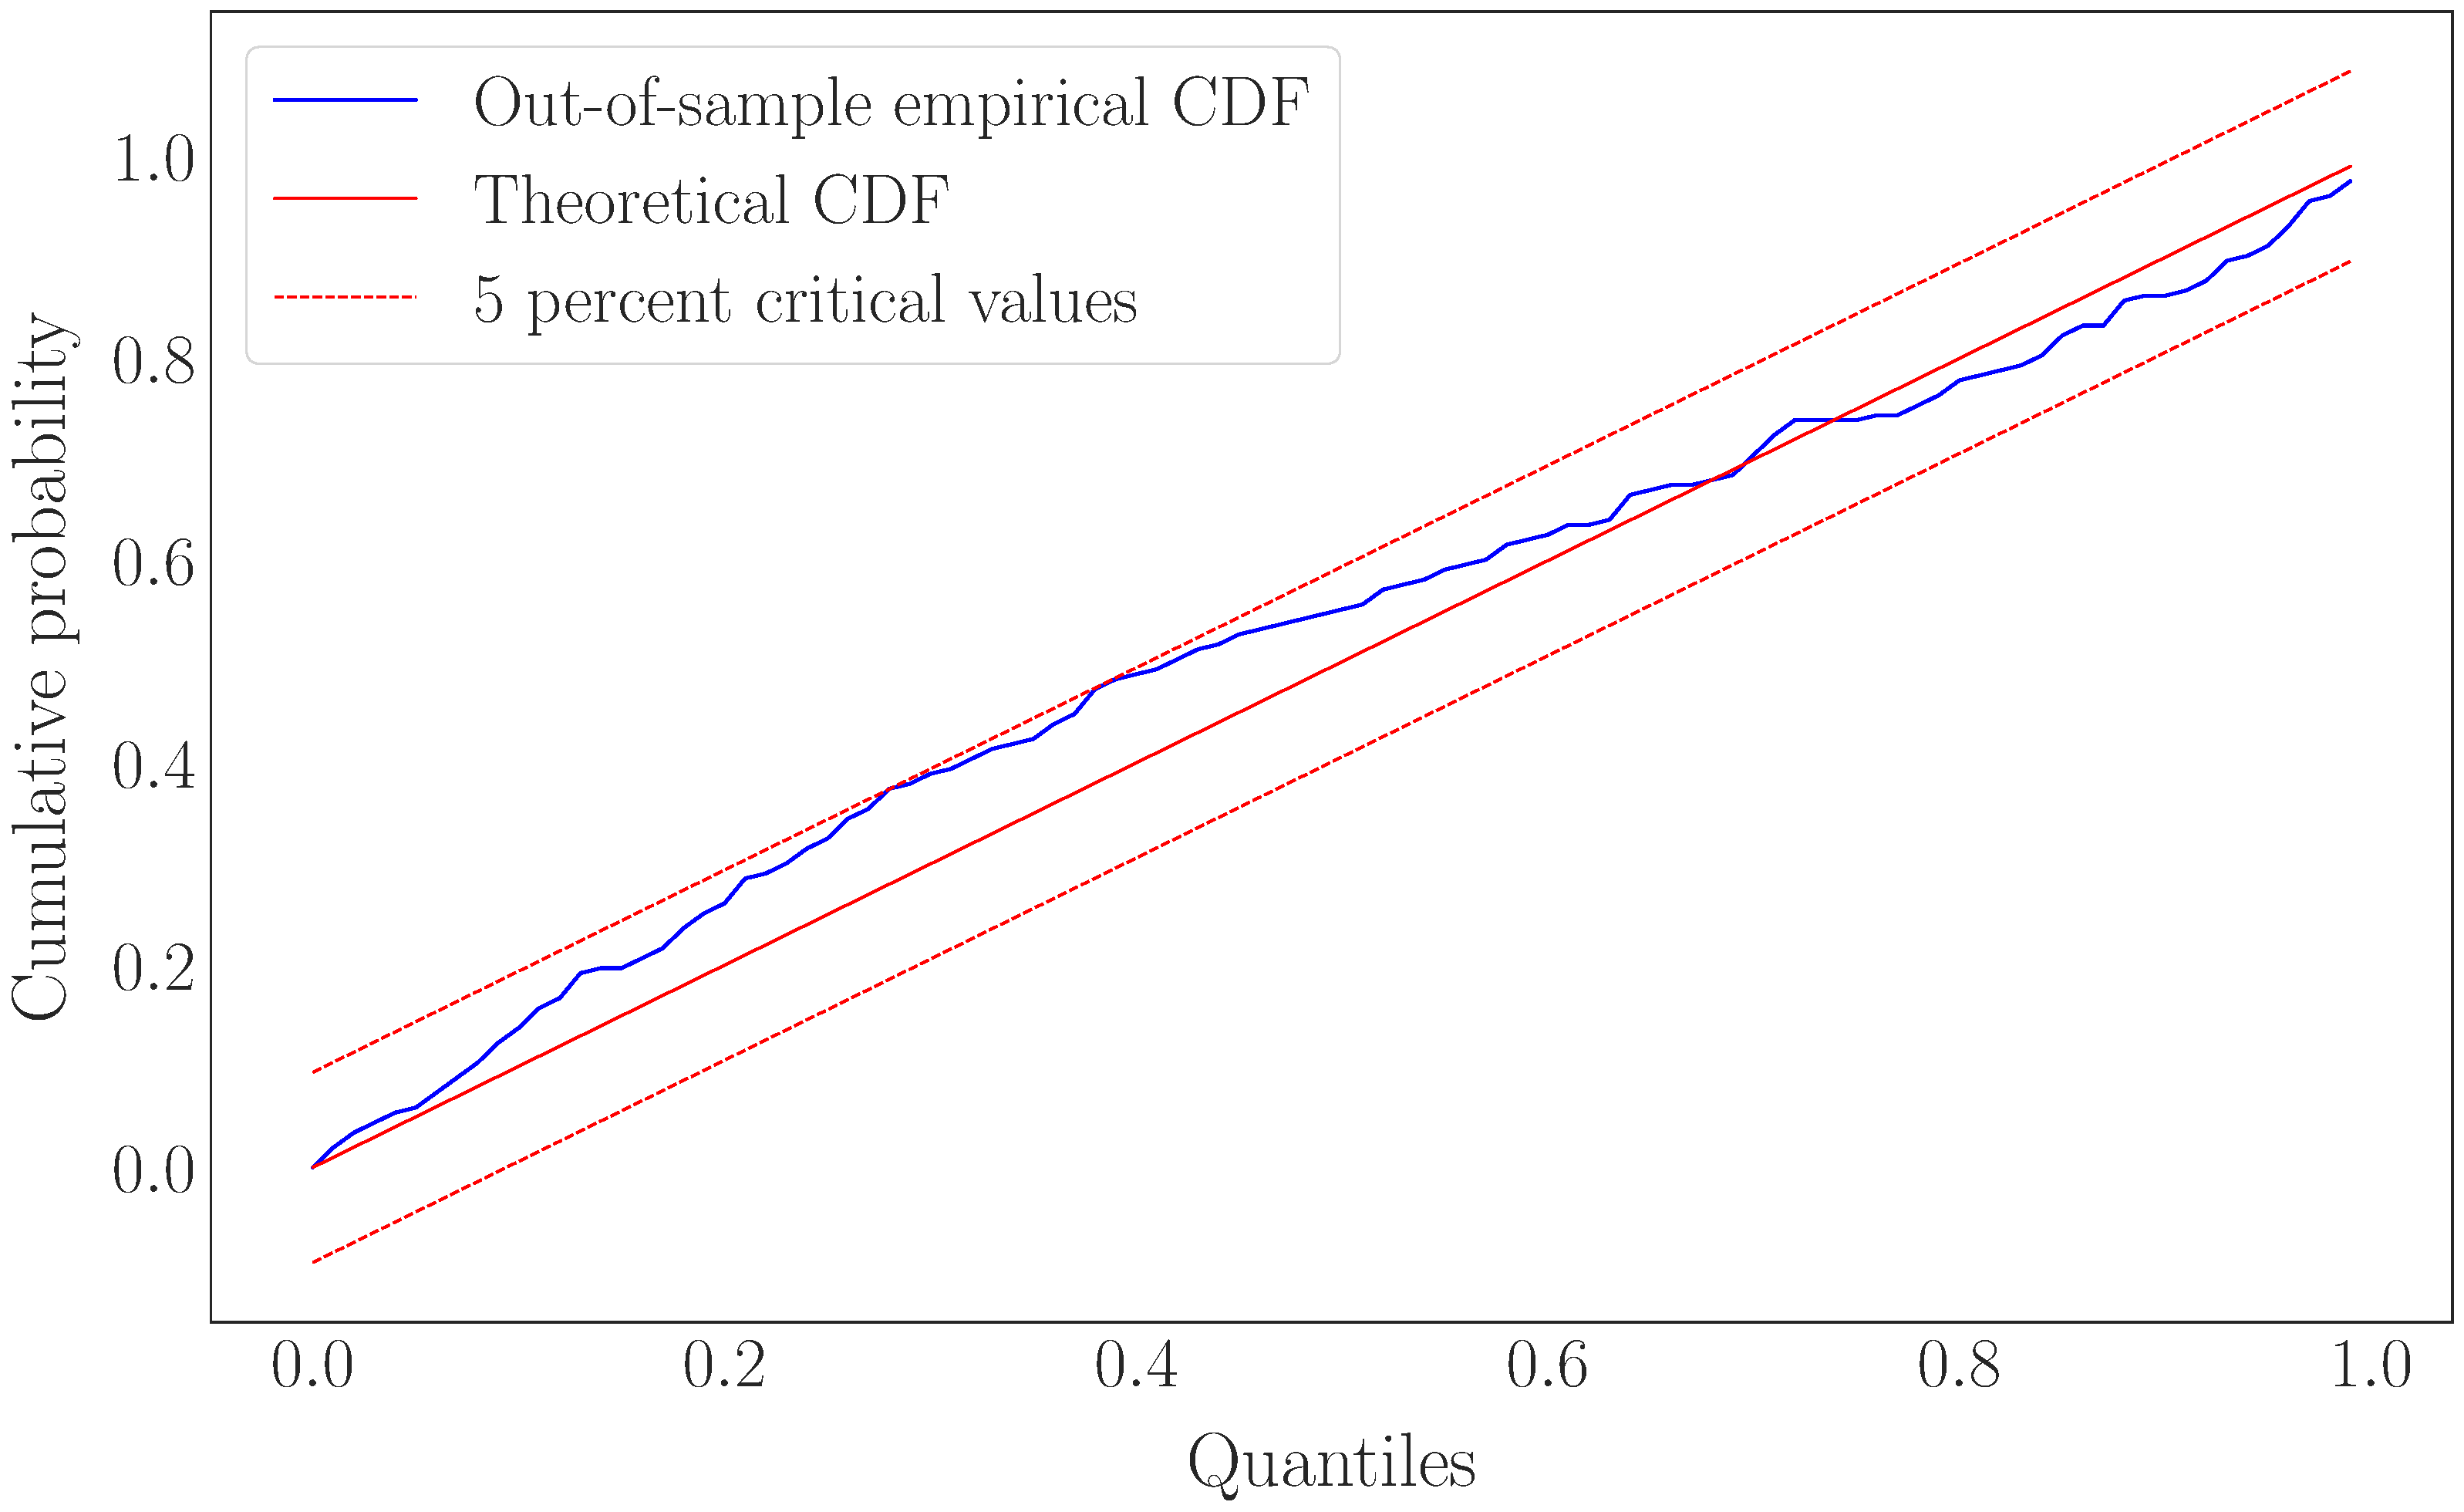
\includegraphics[width=\paperwidth]{img/pitchart.pdf}}
\end{frame}


\begin{frame}
  \frametitle{In Practice}
  \begin{wideitemize}
    \item The package we design handles the optimization seamlessly
    \item It outputs the optimal functional forms and parameters
    \item However, it might be time consuming, given that it involves optimizing over a large number of functional forms
    \item Hence, users might want to re-run the optimization from time to time, but not everytime
      \begin{itemize}
      \item For instance, every month
      \item Or after a structural break, a crisis, etc.
      \end{itemize}
  \end{wideitemize}
\end{frame}


%% ---------------------------------------------------------------------------
%% Benchmarking
%% ---------------------------------------------------------------------------
\section{Benchmarking}

\begin{frame}
  \frametitle{Bank of Mexico FX Interventions Setup}  
  \begin{wideitemize}
    \item The Banco Mexico (BM) implemented both ex-ante, transparent FX
      auctions and discretionary-rate auctions
    \item Different reservation rates:
      \begin{wideitemize}
      \item \textbf{Rule-based setting}: BM operated an auction every day
        with a pre-announced \textbf{a minimum rate} for eligible bids
      \item \textbf{Discretionary setting}: the auction was organized at the BM's discretion without reservation rate
      \end{wideitemize}
  \item Often, no demand for the ruled-based auction as the market rate was
    below the reservation rate
  \item No-minimum price auctions could be motivated by other considerations
    than the exchange rate level
  \item What was the risk level when the FXI occurred?
  \end{wideitemize}
\end{frame}


\begin{frame}
  \frametitle{Rule-Based Benchmarking}
    \makebox[\linewidth]{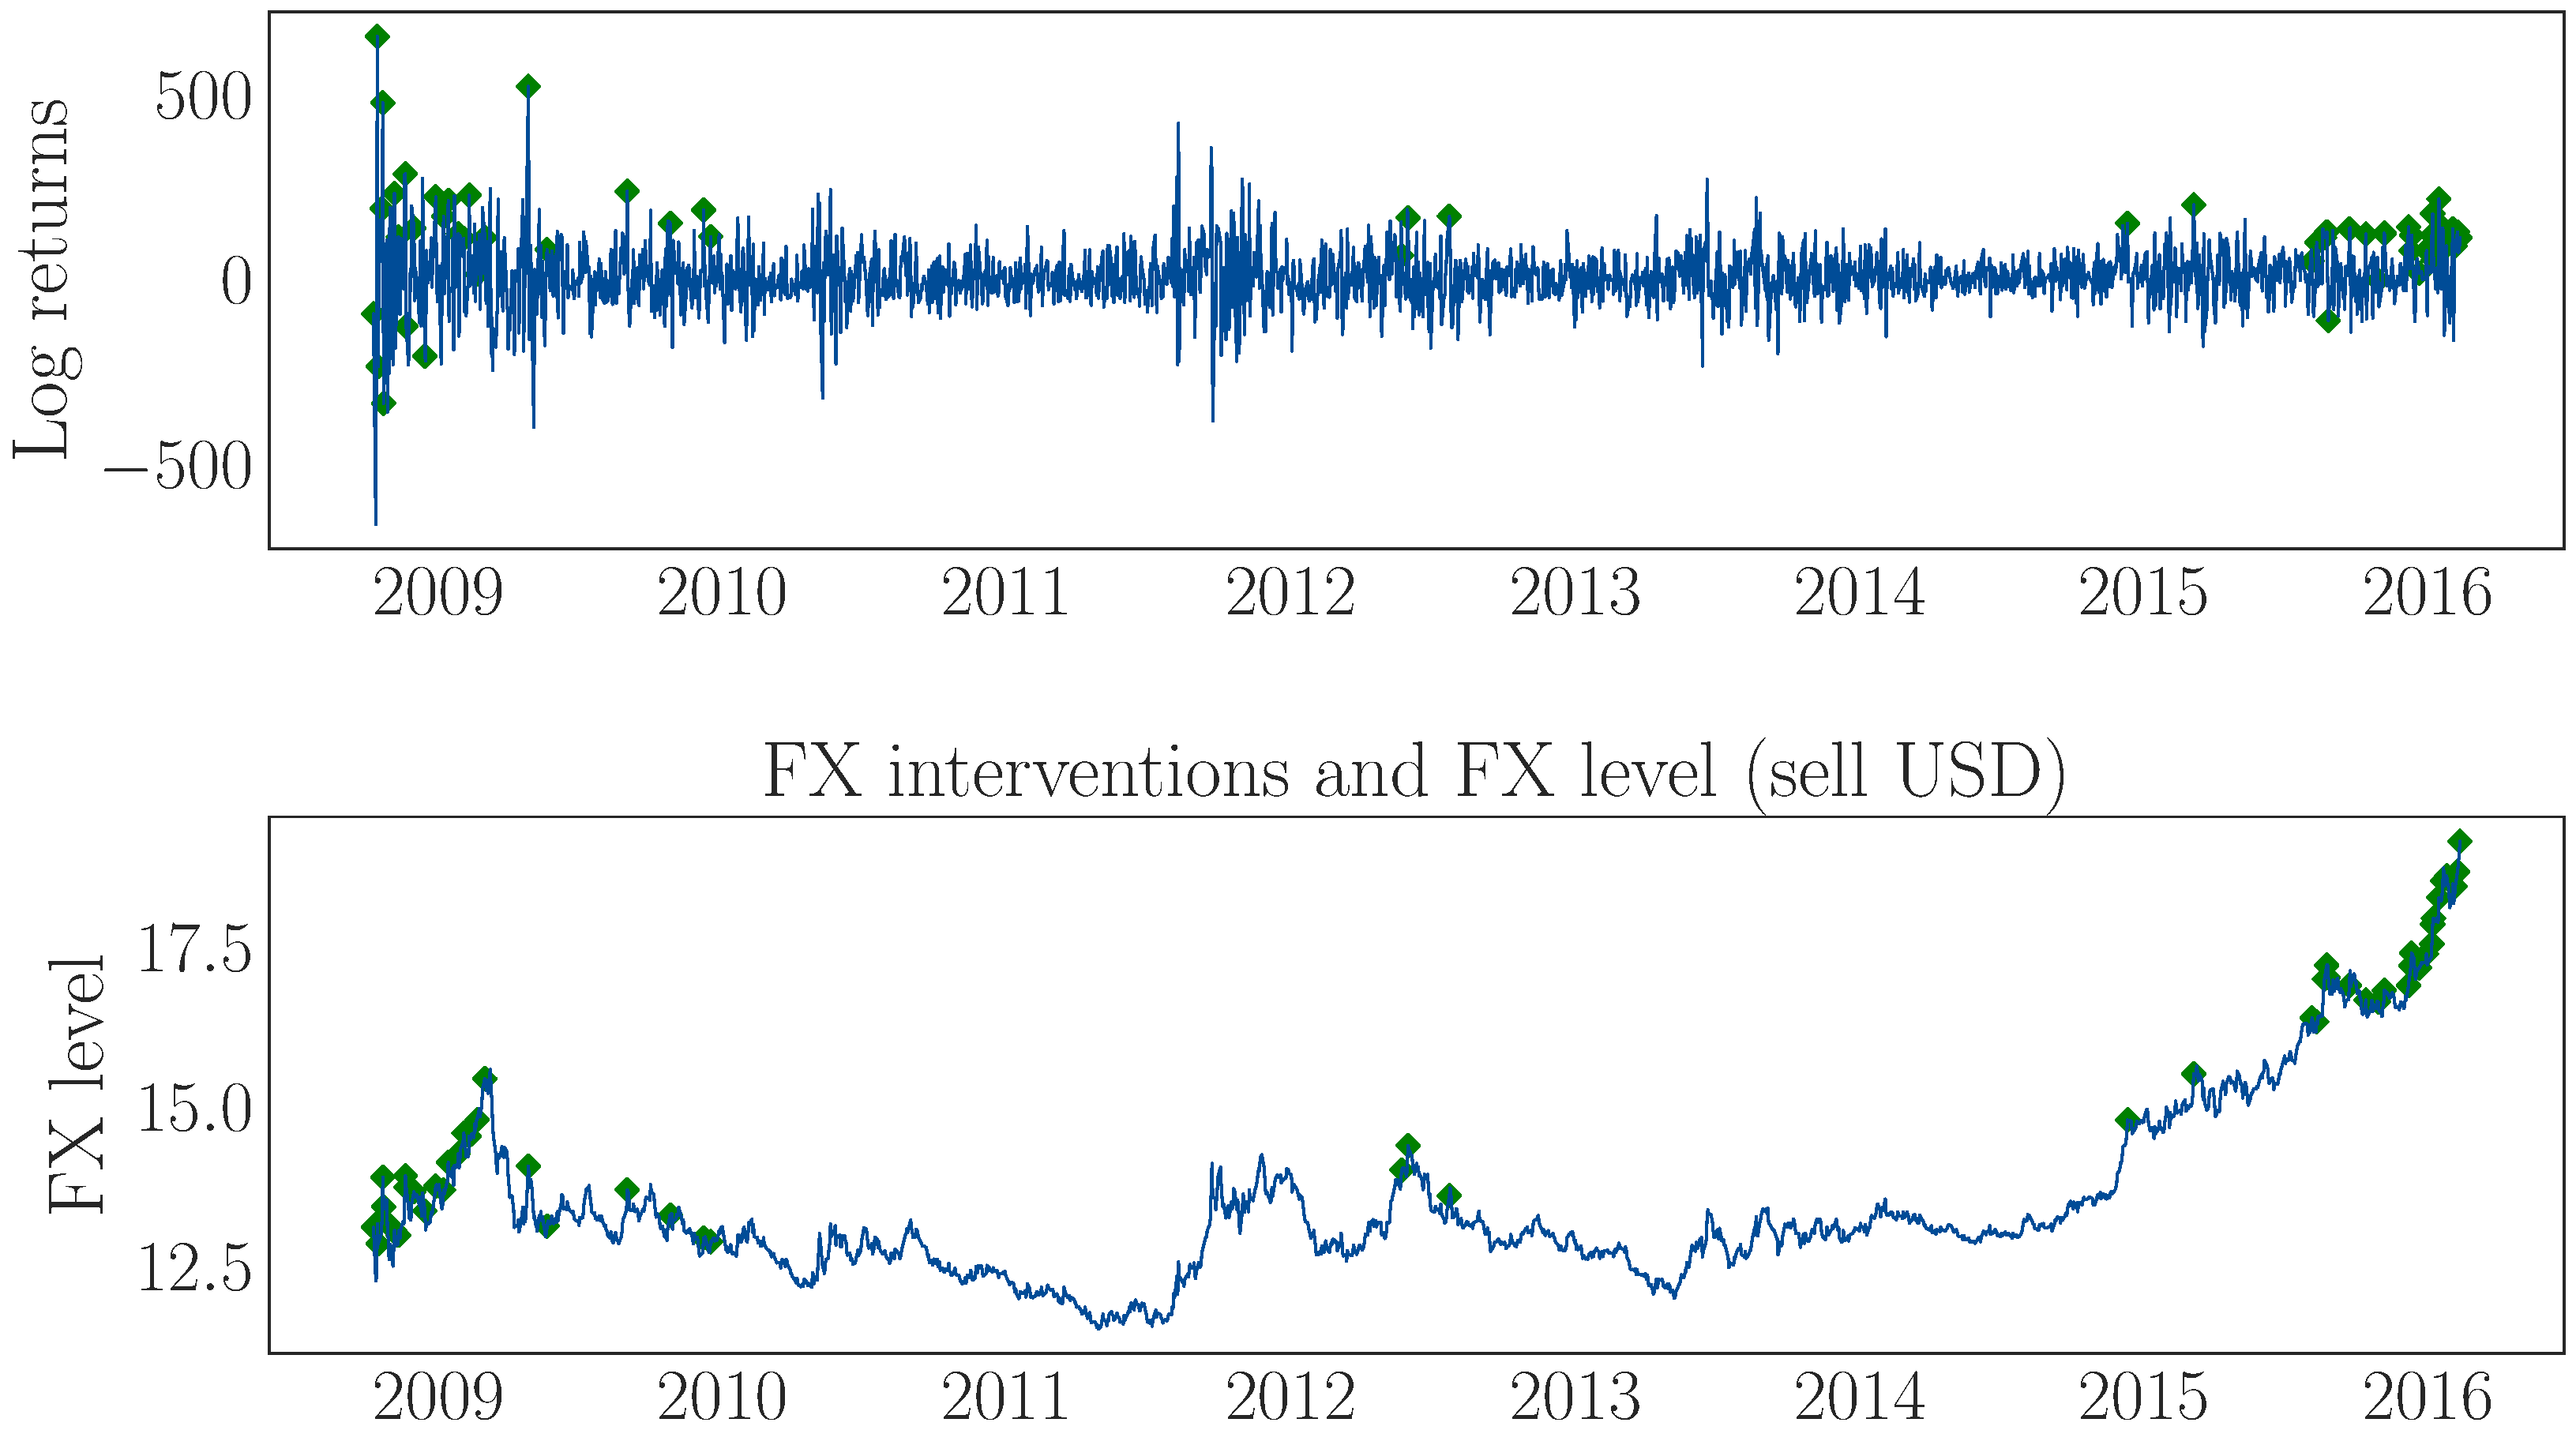
\includegraphics[width=\paperwidth]{img/benchmark_minprice.pdf}}
\end{frame}


\begin{frame}
  \frametitle{Rule-Based Benchmarking: Risk-Level}
    \makebox[\linewidth]{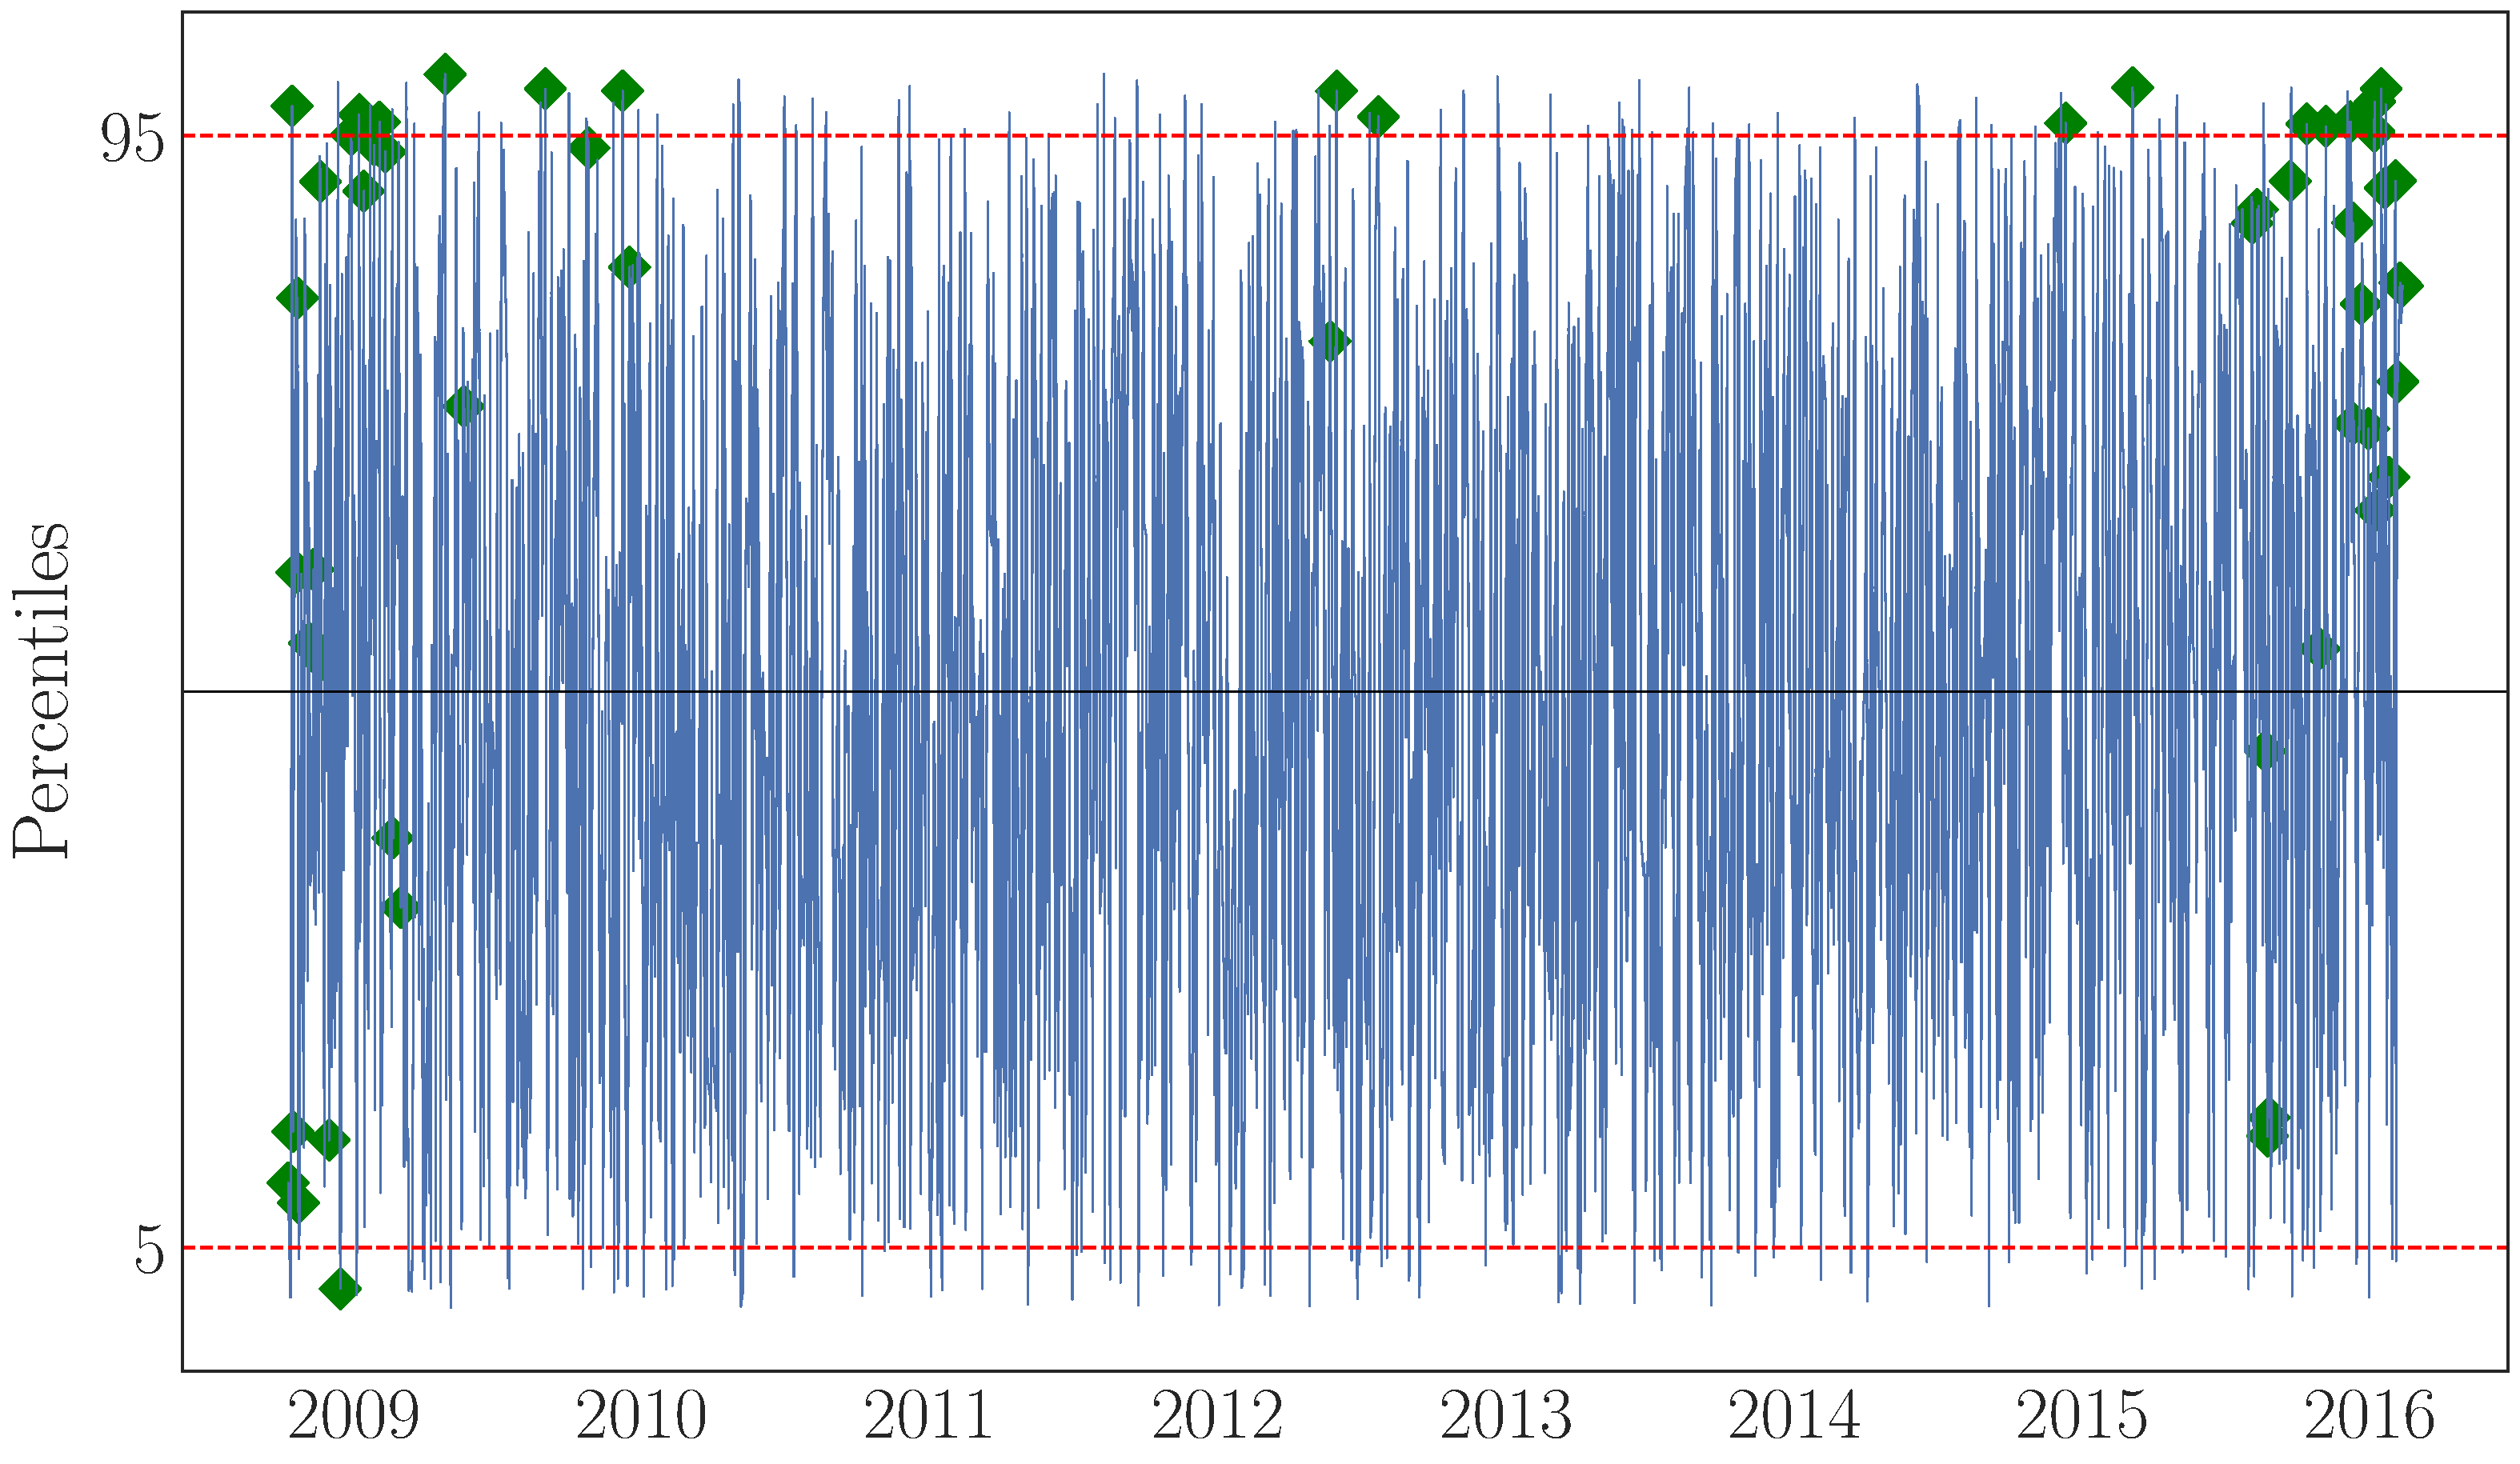
\includegraphics[width=\paperwidth]{img/benchmark_minprice_cdf.pdf}}
\end{frame}


\begin{frame}
  \frametitle{Discretion-Based Benchmarking}
    \makebox[\linewidth]{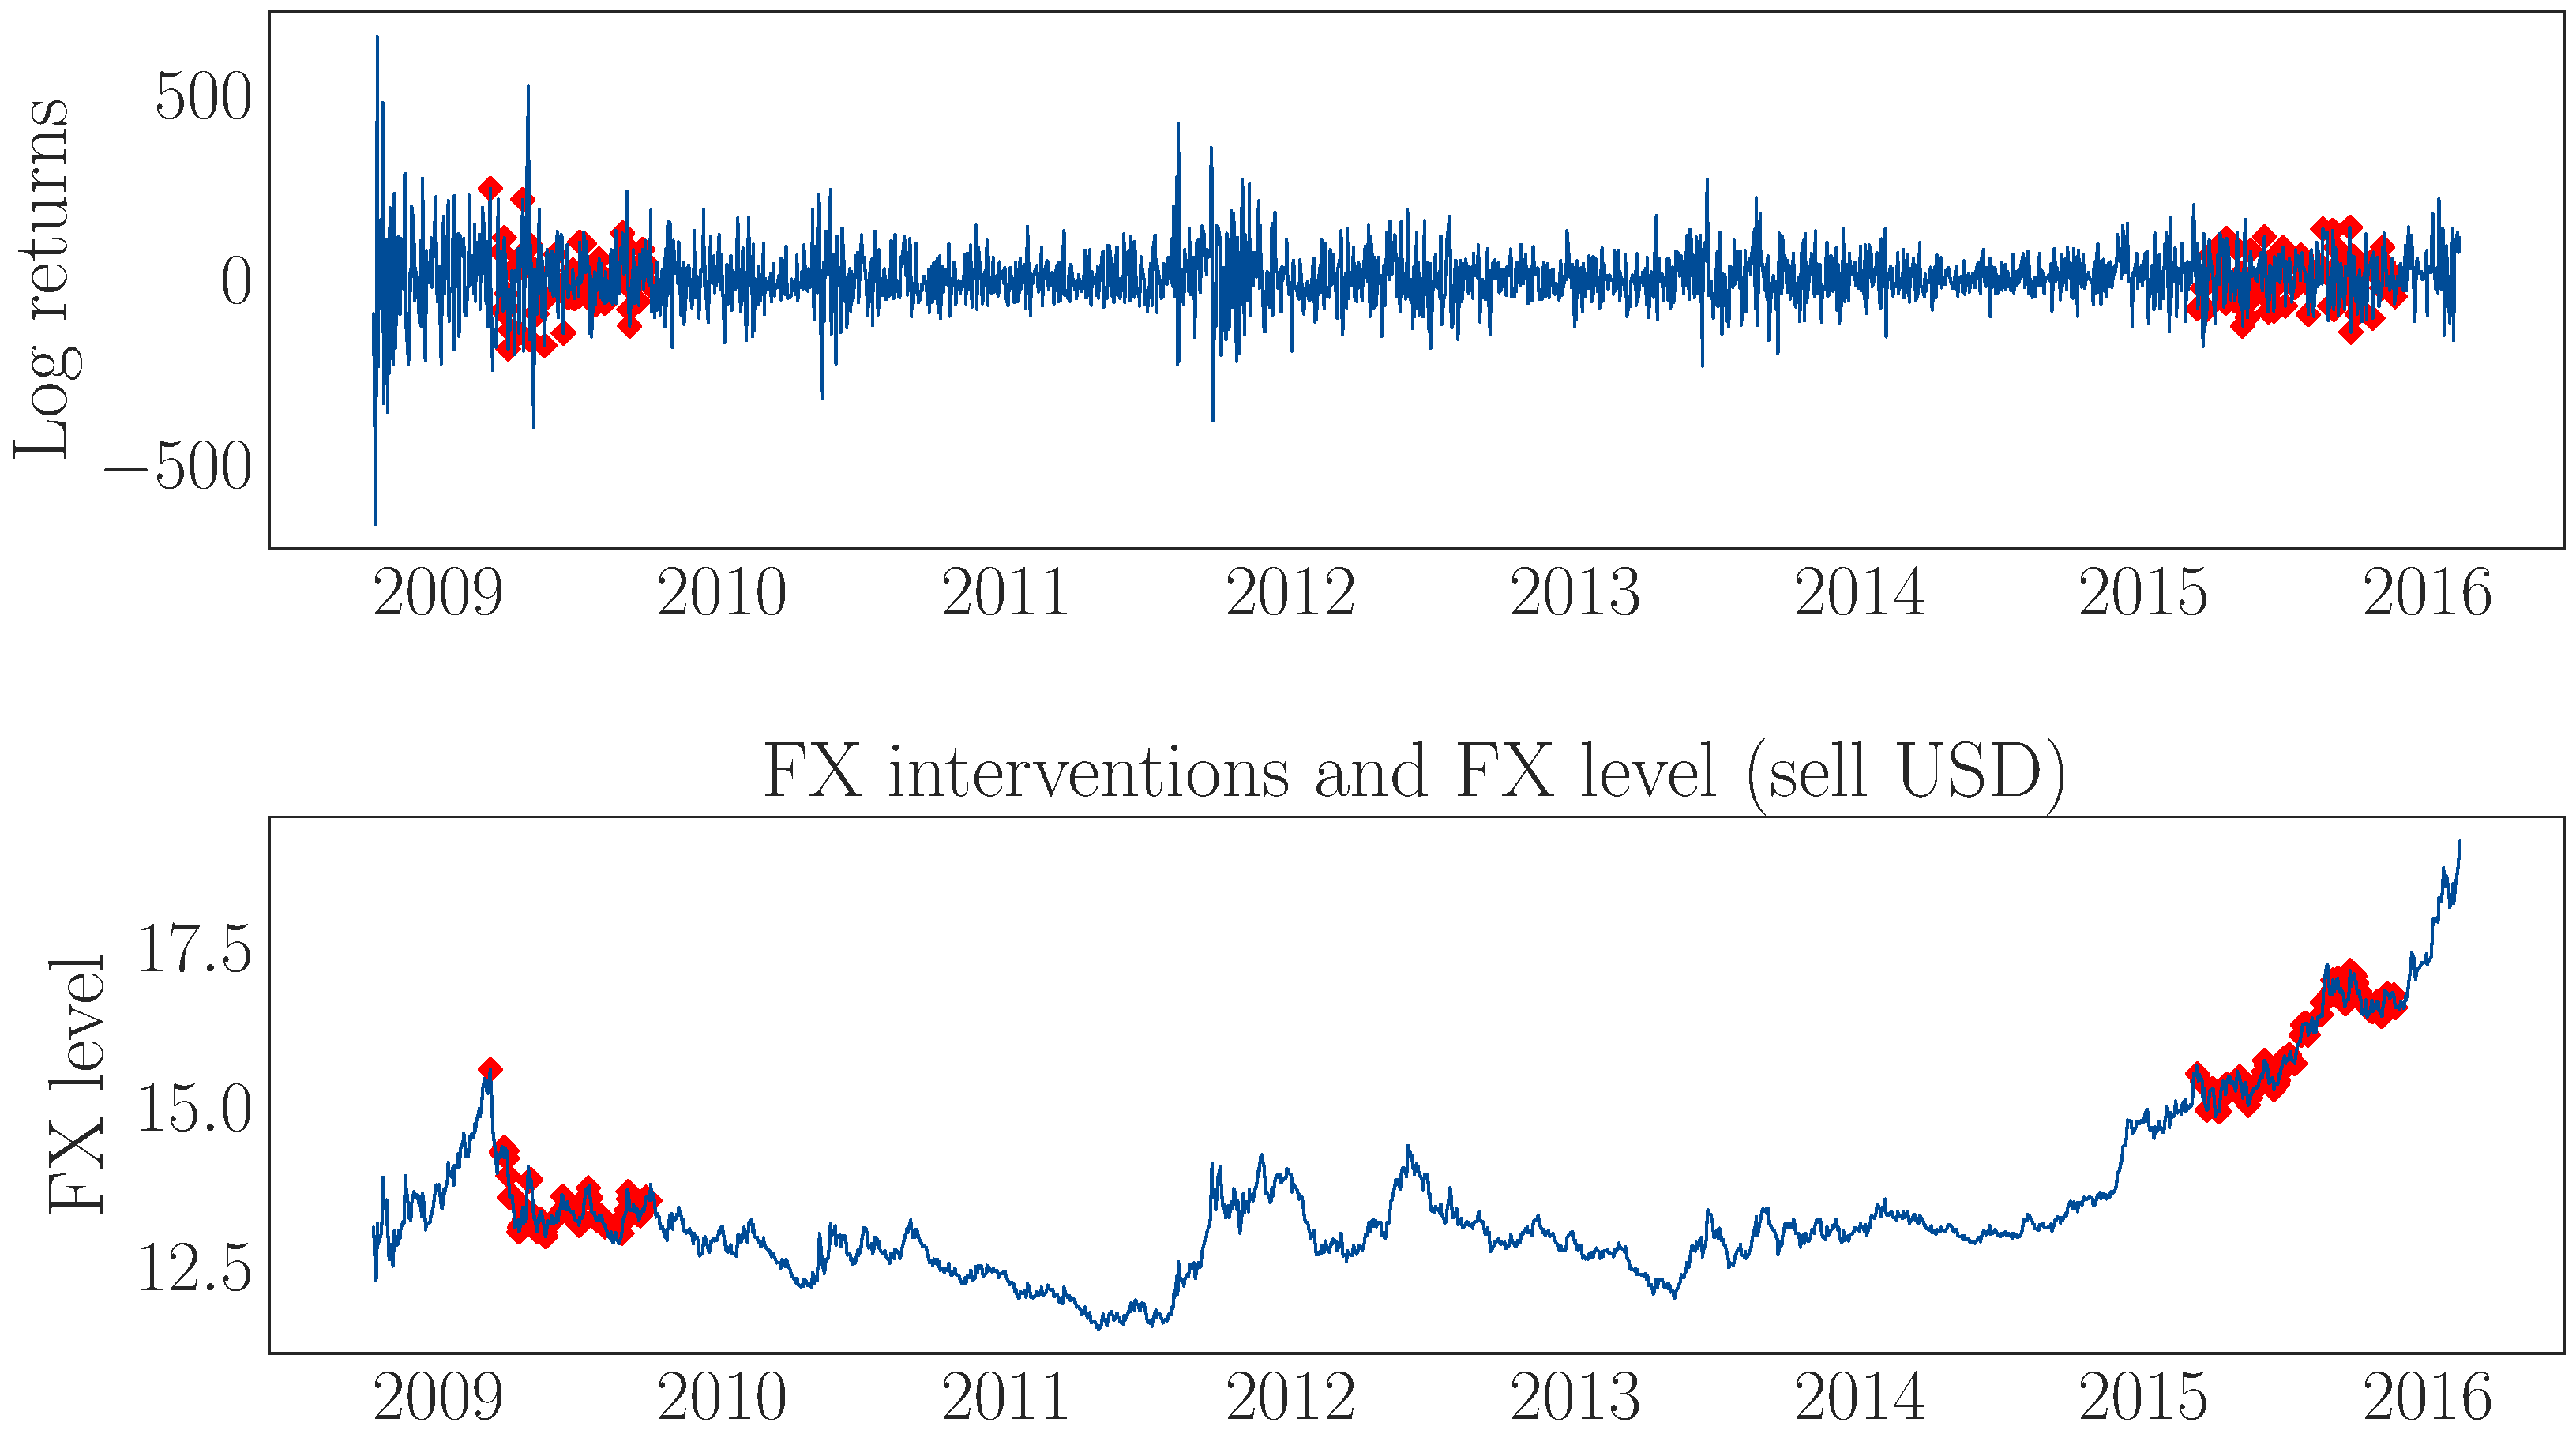
\includegraphics[width=\paperwidth]{img/benchmark_no_minprice.pdf}}
\end{frame}


\begin{frame}
  \frametitle{Discretion-Based Benchmarking: Risk-Level}
    \makebox[\linewidth]{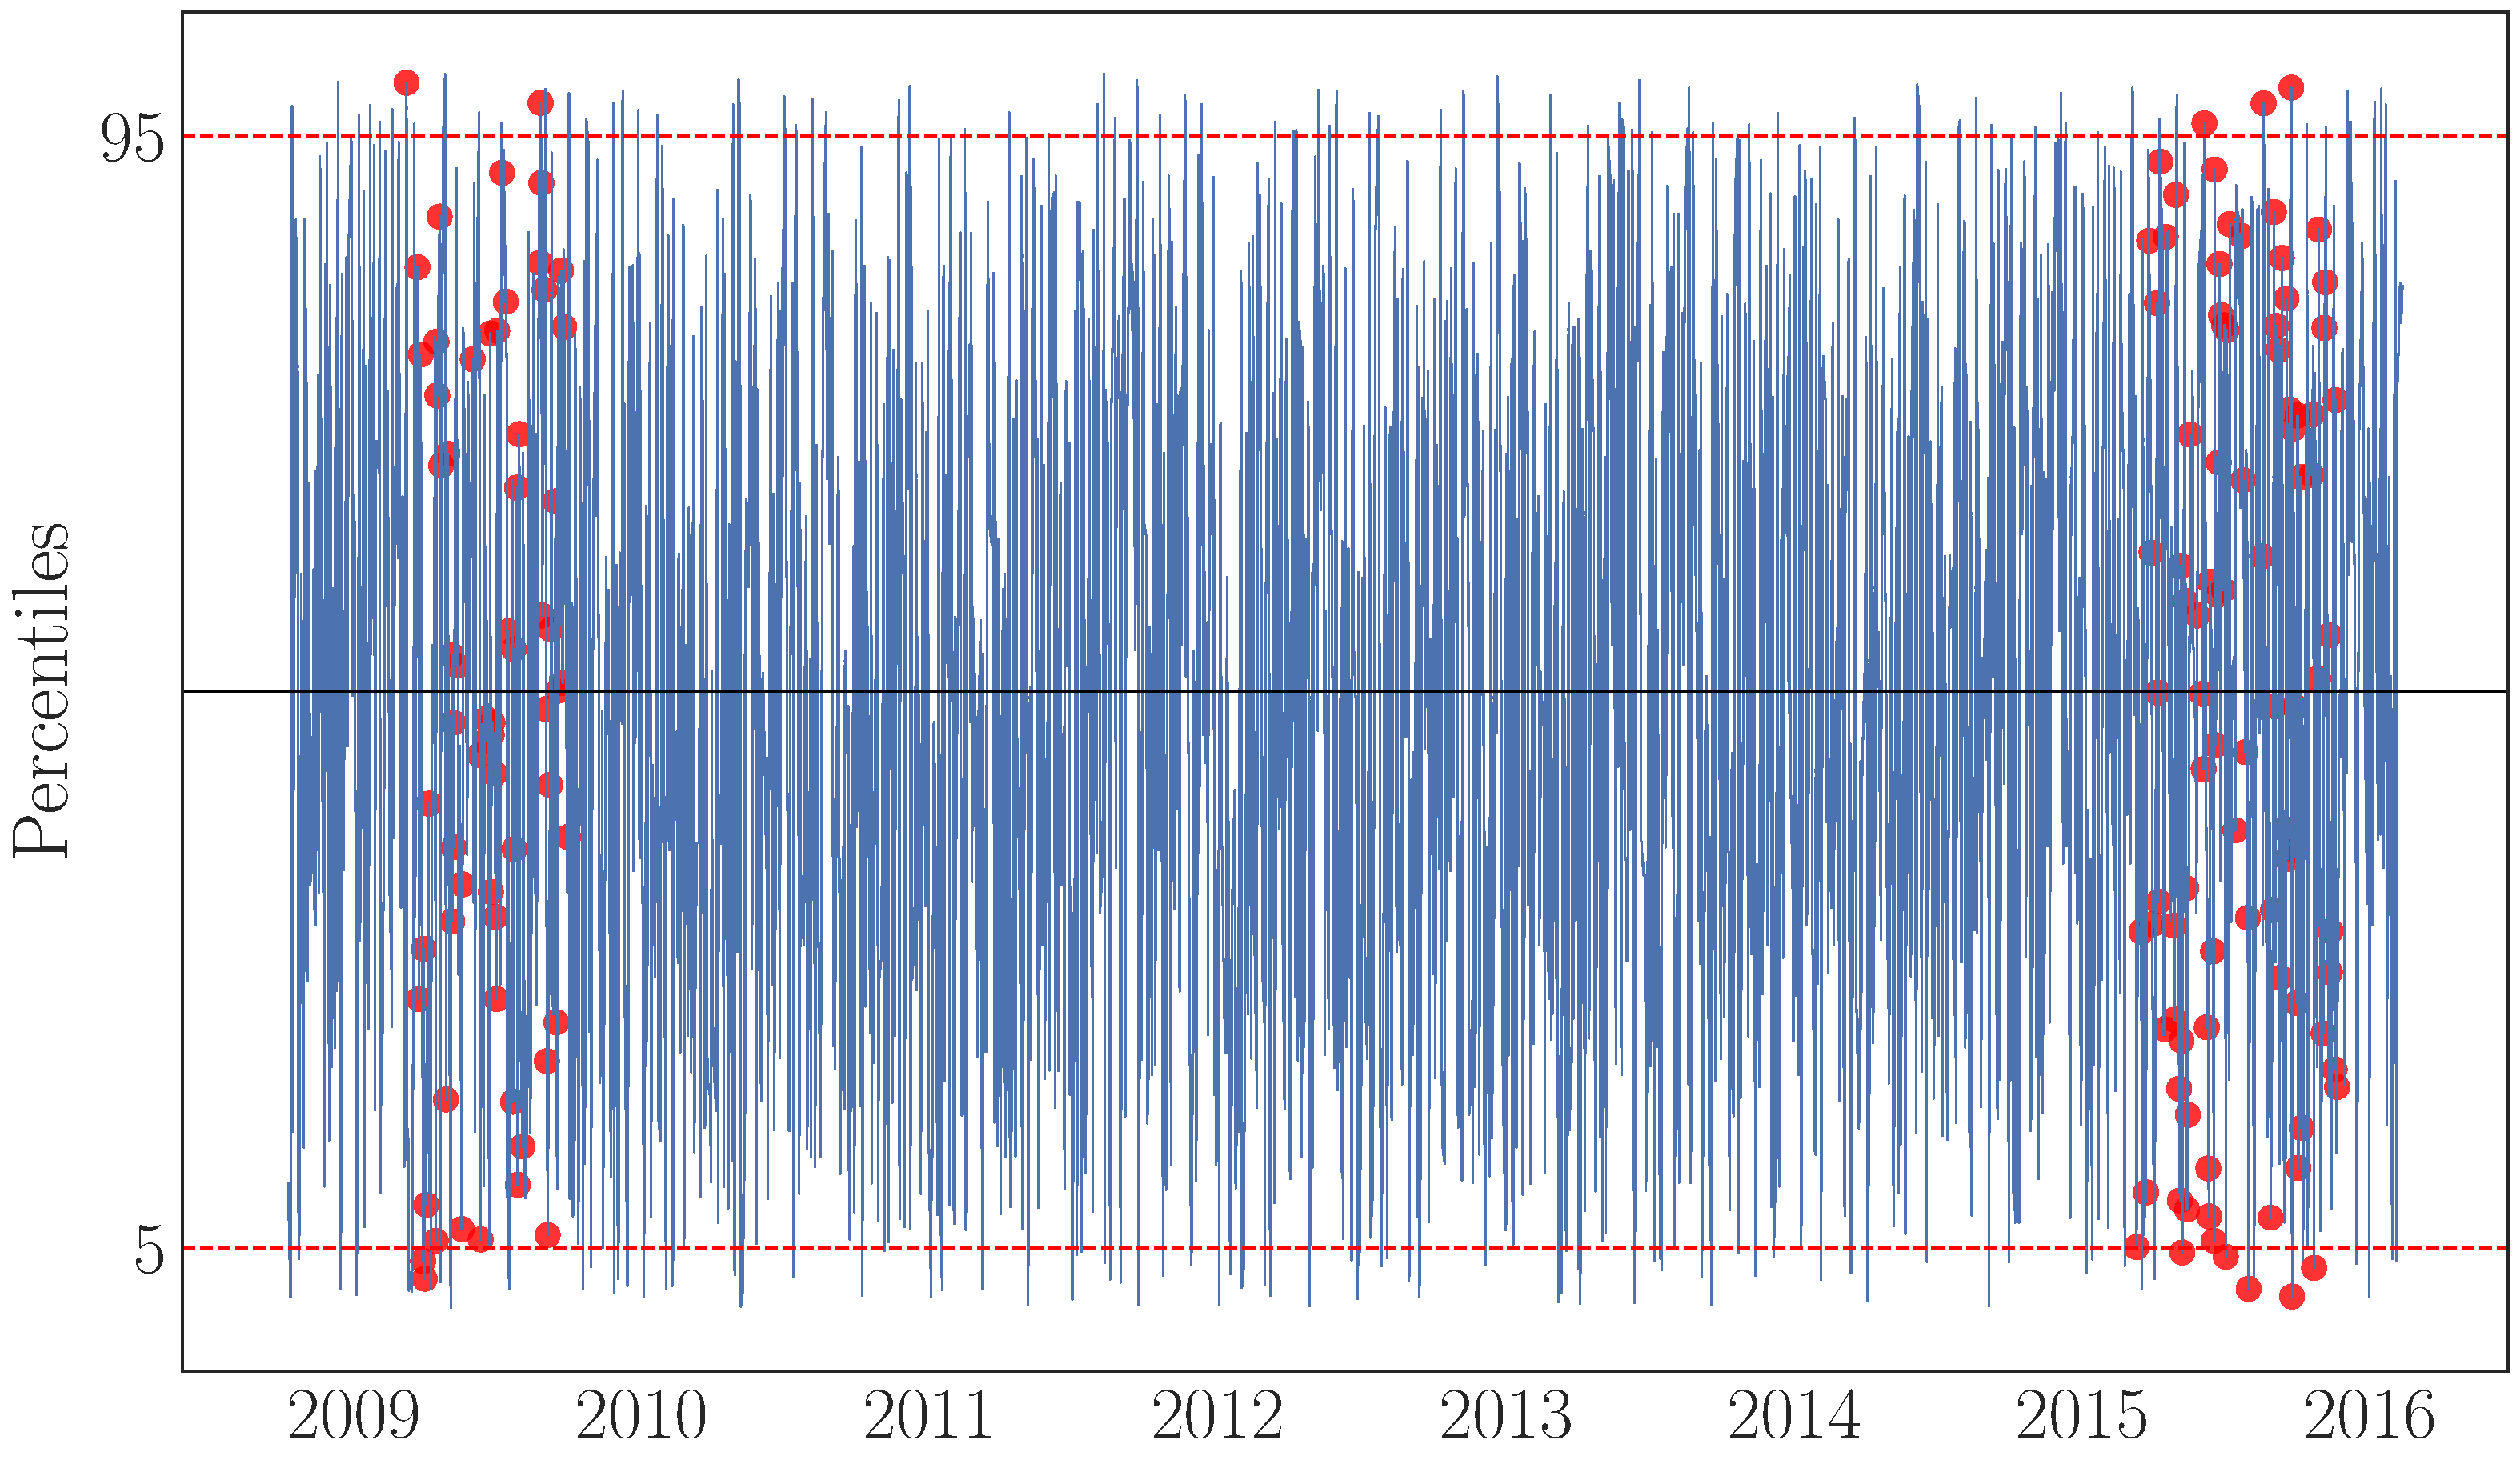
\includegraphics[width=\paperwidth]{img/benchmark_no_minprice_cdf.pdf}}
\end{frame}



\begin{frame}
  \frametitle{Benchmarking Results}
  \begin{wideenumerate}
  \item \textbf{FX auctions with ex-ante minimum price ("rule-based")}
  \begin{wideitemize}
    \item The minimum price auctions did not fully prevented BM to intervene
      outside of the tails of the conditional distribution
    \item In that respect, VaR-based intervention would have been better to
      mitigate tail-risks
    \end{wideitemize}
\item \textbf{FX auctions with no ex-ante minimum price ("discretion-based")}
  \begin{wideitemize}
    \item No minimum prices interventions occurred at almost any risk level
    \item \textbf{Discretion triggers are not identifiable based on risk}
    \end{wideitemize}
  \end{wideenumerate}    
\end{frame}


%% ---------------------------------------------------------------------------
%% Conclusion
%% ---------------------------------------------------------------------------

\section{Policy Uses}

\begin{frame}
  \frametitle{Policy Uses}
  \begin{wideitemize}
   \item Useful for floating rate regimes to \textbf{operationalize their financial
     stability mandate} with a risk-management framework
    \item The VaR-based rule could be considered \textbf{as one option} to improve the
      rules that central banks currently use
    \item Let the nominal exchange rate acts as a \textbf{shock absorber}
    \item Could be used to accompany the \textbf{transition to exchange rate
        flexibility}, with gradually less and less interventions
  \item More generally, could be used by central banks for \textbf{market and risk monitoring}
  \end{wideitemize}
\end{frame}


% \begin{frame}
%   \frametitle{Future Work}
%   \begin{wideenumerate}
%     \item Use expected shortfall (ES) instead of VaR, as ES has better risk
%       properties
%     \item Look \textbf{beyond spot FX markets} and apply a similar and consistent
%       approach to:
%       \begin{itemize}
%       \item FX derivatives, e.g. forward spreads
%       \item Offshore/onshore interest
%         rate markets
%       \item Fixed income market 
%       \end{itemize}
%    \item Determine the risk tolerance by \textbf{identifying vulnerabilities} and their
%      impact to the economy. Align with the "\textbf{at-risk}" work done in MCM
%   \end{wideenumerate}
% \end{frame}


\begin{frame}{Alternative Models: Benchmarking}
\setlength\tabcolsep{2pt}  % default value: 6pt
\tiny  %%  command to change the font size
\begin{tabular}{llll}
\toprule
{} &   PIT & Logscore diff against Baseline & Diff pvalue \\
\midrule
Baseline        &  Pass &                                &             \\
Unconditional   &       &                                &             \\
Quantile Reg    &       &                                &             \\
Gaussian EGARCH &  Fail &                           1.54 &       0.938 \\
TSkew GARCH     &  Fail &                          1.768 &       0.961 \\
Gaussian GARCH  &  Fail &                          1.755 &        0.96 \\
\bottomrule
\end{tabular}

\normalsize
\end{frame}



%% ---------------------------------------------------------------------------
%% End document
%% ---------------------------------------------------------------------------
\end{document}


%%% Local Variables:
%%% mode: latex
%%% TeX-master: t
%%% End:
